\section{Introduction}

\noindent The \CENTREX\ experiment aims to employ a molecular-beam resonance
technique to measure the nuclear Schiff moment of $^{205}\Tl$ in thallium
fluoride as a test of physics beyond the Standard Model. In the following, I
outline the motivation from $CP$-violation and baryon asymmetry, define the
Schiff moment and suggest how it can be measured. After reviewing relevant
features of the TlF molecule, we present previous experiments as well as the
measurement scheme proposed in this work.

\textit{Note: This chapter served as the first draft of our overview paper
\cite{grasdijk2021centrex} and as such contains a lot of the same information.}

\subsection{Motivation}

Before the early 1960s, it was believed that $CP$ is a good symmetry of nature.
Landau pointed out that that would make it impossible for fundamental particles
to have electric dipole moments along their spin axes
\cite{landau1957conservation}. In a letter published in 1950, Purcell and Ramsey
\cite{purcell1950possibility} stated they are undertaking an experiment to
directly measure, or set a limit on, the neutron \gls{EDM} experiment. Indeed,
were such an \gls{EDM}\ to be detected, that would provide clear evidence of
\gls{CPV}.

It has been found since that while most processes preserve $CP$, certain
flavor-changing decays of heavy mesons violate it as observed in neutral $K$
decays at the 0.003 level \cite{christenson1964evidence} and in other systems,
where it can be as high as 0.7 \cite[chapter 13]{PDG16}. To account for the
experimental evidence, the flavor-changing part of the standard model quark
sector includes a \gls{CPV}\ phase in the \gls{CKM} quark-mixing matrix.
\cite{peccei1995} This so-called Kobayashi--Maskawa mechanism, which introduced
the third quark generation precisely to explain \gls{CPV}\
\cite{kobayashi1973cp}, agrees with all particle physics experiments to date.
\cite{hou2011source}

No corresponding flavor-neutral \gls{CPV}\ has been observed yet. In principle,
the \QCD\ Lagrangian could contain a term of the form
\cite[eqn~1]{pospelov1999theta}
%
\begin{equation}
   \L = \theta
   \frac{g^2}{32\pi^2}G_{\mu\nu}^a\widetilde{G}^a_{\mu\nu},
\end{equation}
%
where $\theta$ is called the vacuum angle or simply the $\theta$-parameter, $g$
is the gauge coupling parameter for the strong force, $G^a$ is the gluon field
tensor, and $\widetilde{G}^a_{\mu\nu}=\frac12\epsilon^{mn}_{\mu\nu}G^a_{mn}$ is
its Hodge dual \cite[eqn~2.82]{carroll2004spacetime}, defined in terms of the
Levi-Civita tensor $\epsilon^{mn}_{\mu\nu}$. Experimental evidence from searches
for the \gls{EDM} of neutral $^{199}$Hg atoms \cite{graner2016reduced} and
neutron \gls{EDM}\ experiments \cite{baker2006improved} suggests that the
strength of this term relative to the usual strong interaction is limited to
$|\theta|<10^{-10}$. Presently accepted theories cannot explain why $\theta$
should be that small; this fine-tuning issue is known as the strong $CP$
problem. See \cite{graham2015experimental} for a brief review of a few possible
solutions.

At present, searches for \glspl{EDM} give the most sensitive constraints on
flavor-diagonal \gls{CPV}. Conversely, given a particle physics model with
\gls{CPV}\ we can predict what the expected \gls{EDM}\ of the particles is. For
example, in the Standard Model, the \gls{CKM} phase can produce a lepton
\gls{EDM}\ no larger than $10^{-38}\,e\cm$. Part of the reason the electron
\gls{EDM}\ is so suppressed is that it cannot appear below the four-loop level.
\cite{pospelov1991electric} In comparison, the quark \gls{EDM} can be induced at
the three-loop level \cite[sect~4.1.1]{pospelov2005electric}. For example, the
\gls{EDM} of a down quark has been estimated as $10^{-34}\,e\cm$
\cite[eqn~4.75]{pospelov2005electric}, and for the neutron, $10^{-32}\,e\cm$
\cite[eqn~4.76]{pospelov2005electric}. Given how small these effects are in the
Standard Model, \glspl{EDM} thus provide nearly background-free evidence of new
physics.

In order to facilitate the comparison of \gls{EDM} experiments to other
developments in moden physics, we can relate the \gls{EDM} experimental
sensitivity to the energy scale at which new physical phenomena could be
expected to take place. Pospelov and Ritz
\cite[sect~4.1.3]{pospelov2005electric} estimate that at the time of their
writing (2005), the experimental \gls{EDM} sensitivity corresponds to an energy
scale of $10^{6}\GeV$, while the \gls{CKM} background discussed in the previous
paragraph would only become apparent when probing effects beyond the energy
scale of $10^{11}\GeV$.

The second major motivation for searching for new \gls{CPV} physics comes from
the \gls{BAU}. Compared to the current number density of photons in the universe
($n_\gamma \approx411\cm^{-3}$), the current baryon density
($n_\text{B}\approx2.54\cdot 10^{-7}\cm^{-3}$) is some $1.6\cdot10^{9}$ times
smaller \cite[Table 17]{bennett2013nine}. In contrast, the antibaryon density
$n_{\bar{\text{B}}}$ is smaller still; the range of upper bounds for the
antimatter-to-matter number ratio has been reported as $10^{-15}$ to $10^{-6}$
\cite{canetti2012matter}. We should note that the antimatter-to-matter ratio
tends not to be used as a measure of \gls{BAU}; instead, authors tend to prefer
the ratio
%
\begin{equation}
\eta =
    \frac{n_\text{B}-n_{\bar{\text{B}}}}{n_{\gamma }}
   \approx
    \frac{n_\text{B}}{n_{\gamma }}
   \approx 10^{-10}.
\end{equation}

There is as of yet no commonly accepted baryogenesis mechanism, i.e.,
explanation for how the imbalance between the number of particles and
antiparticles came to be. In a 1967 paper \cite{sakharov1991violation}, Sakharov
hypothesized that \gls{CPV}\ is necessary to explain the present
imbalance---which he calls `$C$ asymmetry'---if we assume the initial conditions
of the universe were $C$-symmetric.

However, it is claimed that the `amount' or the `strength' of \gls{CPV}\ in the
\gls{CKM} matrix is not enough to explain the extent of the current \gls{BAU}. A
common argument to this effect compares the size of the dimensionless constants
used to parametrize the two effects. For \gls{BAU}\ we have
$\eta\approx10^{-10}$ as defined above, whereas for \gls{CPV}\ the constant is
no larger than $10^{-20}$ \cite[sect 2.3]{riotto1999recent}. The latter number
refers to the \gls{CPV}\ invariant that can be defined in terms of quark masses
as \cite[eqn~3]{hou2011source}
%
\begin{equation}
   J = A(m_\text{t}^2 - m_\text{u}^2)
        (m_\text{t}^2 - m_\text{c}^2)
        (m_\text{c}^2 - m_\text{u}^2)
        (m_\text{b}^2 - m_\text{d}^2)
        (m_\text{b}^2 - m_\text{s}^2)
        (m_\text{s}^2 - m_\text{d}^2),
\end{equation}
%
where $A$ is twice the area of any ``unitarity triangle'' (the six possible
triangles all have the same area) of the \gls{CKM} matrix (see \cite[fig
12.1]{PDG16}). With quark masses from \cite[p40, ``Quark Summary Table'']{PDG16}
and $A\approx3\cdot10^{-5}$ from \cite[p7]{kleinknecht2006unitarity}, we get
$J\approx121\cdot 10^3\GeV^{12}$.  The electroweak phase transition, occurring
at temperature $T_\text{EW}\approx100\GeV$, was the latest point in the
evolution of the universe when \gls{BAU}\ could have been generated
\cite{fodor2000EW}. Comparing $J$ and $T_\text{EW}$, we get the desired
dimensionless quantity $J/T_\text{EW}^{12}\approx10^{-20}$ to within factors of
order unity. It is ten orders of magnitude smaller than the constant
parametrizing the baryon asymmetry. Thus, new sources of \gls{CPV}\ are needed.

More sophisticated analyses agree with this basic conclusion. For example,
Tranberg et al.\ \cite[eqn~20]{tranberg2010cold} calculate that in the standard
model, the baryon asymmetry has the value
%
\[
    \frac{n_\text{B}}{n_\gamma}=0.978\times(4.4\pm1.9)\times10^{-6},
\]
%
which is four orders of magnitude larger than the observed asymmetry.

\subsection{Schiff moment}

Additional $T$-violating forces would likely give rise to a nuclear \gls{EDM},
whether through the \gls{EDM}\ of unpaired protons or neutrons, via \gls{CPV}\
interactions between valence nucleons and the core of the nucleus, or other
mechanisms \cite{safronova2018search}. The \gls{EDM}\ $\vec d$ would result from
a redistribution of nuclear charge density and would violate $T$, as follows.
Since the nuclear spin $\vec I$ is the only preferred direction in a nucleus,
the dipole moment also has to point along it: $\vec d=d\vec I/I$. Under
time-reversal, the \gls{EDM}\ would stay the same but the spin would flip direction.

However, according to the Schiff theorem, an \gls{EDM}\ of a nonrelativistic
point nucleus would not be observable outside of a neutral atom or molecule
containing the nucleus. More precisely, the interaction energy of
nonrelativistic point charged electric dipoles in an arbitrary external
electrostatic potential has no term linear in the \gls{EDM} if the dipoles are a
part of a bound, electrically neutral collection of particles
\cite{schiff1963measurability}. Physically, the system rearranges itself so as
to screen the external field completely \cite[p33]{safronova2018search}. Thus, a
$T$-violating \gls{EDM}, if existent, would be very hard to detect
experimentally without a mechanism to bypass Schiff's theorem.

In the following, we work out the shielding of a nuclear \gls{EDM}\ in an atom
with a Hamiltonian $\hat H$. In particular, this simple model does not attempt
to take into account the complexity of molecular structure. The argument
consists of the following steps: (1) Write down the atomic Hamiltonian $\hat H$.
(2) Extract $T$-odd terms from the multipole expansion of $\hat H$. (3) Show
that for a point nucleus, these terms can be written as a commutator $[\hat
H,\ldots]$ and thus have a vanishing expectation value and no corresponding
linear energy shift. (4) Relax the point-nucleus assumption, and find the
residual (unscreened) interaction. To find the expectation value (or the linear
energy shift) due to the interaction, two conditions need to be satisfied: the
atom needs to be polarized by an external electric field (step 5), and the
interaction needs to have a nonzero matrix element between states of opposite
parity (step 6). Finally, we interpret $\vec S$ in terms of nuclear electric
field (step 7).

\paragraph{Step 1: Atomic Hamiltonian}

Consider an atom of proton number $Z$ in an external electric field $\vec E_0$,
with electrons of momenta $\vec p_i$ at positions $\vec r_i$, and a nucleus with
the charge distribution $\rho(\vec R)$. The atom's Hamiltonian includes the
following interactions:
%
\begin{align*}
    \hat H\;=\quad
    &\sum_{i=1}^Z\frac{\vec p_i^2}{2m}
        \tag{electron kinetic energy}\\
    +\frac{1}{2}&\sum\limits_{i,j}\frac{e^2}{|\vec r_i-\vec r_j|}
        \tag{electron--electron}\\
    -Ze^2&\sum_i\int\frac{\rho(\vec R)\d^3\vec R}{|\vec r_i-\vec R|}
        \tag{electron--nucleus}\\
    +e&\sum_i\vec r_i\cdot\vec E_0
        \tag{electrons in external field}\\
    -Ze&\ex{\vec R}\cdot\vec E_0.
        \tag{nuclear dipole in external field}
\end{align*}
%
Note that this Hamiltonian is not expressed in SI units.

The nuclear charge density is normalized to $\int\rho(\vec R)\d^3\vec R=1$.
Almost all the integrals in this section are weighted by $\rho(\vec R)$,
suggesting the use of the measure $\dd^3(\vec R)\equiv\rho(\vec R)\d^3(\vec R)$.
Thus we have the dipole moment $\ex{\vec R}\equiv\int\vec R'\dd^3\vec R'$;
later, we shall also make use of the third moment $\ex{R^2\vec R}\equiv\int
(R')^2\vec R'\dd^3\vec R'$.

The interaction of the nuclear monopole with the external electric field does
not appear in the Hamiltonian as it corresponds to a mere constant offset.
Interacting with the external field, the nuclear charge distribution gives rise
to the dipole term $-e\ex{\vec R}\cdot\vec E_0$, while higher moments of
$\rho(\vec R)$ do not contribute when the external field $\vec E_0$ is uniform.

\paragraph{Step 2: Extract $T$-odd terms}

First we show that odd-parity moments, such as the \gls{EDM}, violate both $T$
and $P$. Any $2^\ell$-pole moment, for $\ell\in\mathbb{N}$, is a rank-$\ell$
tensor and as such must be aligned with a rank-$\ell$ tensor made from the spin
operator $\vec I$. For example, the quadrupole moment is the rank-2 tensor
$Q_q\propto T^2(\vec I,\vec I)_q$. This explains why nuclear electric quadrupole
moment is not exotic: it does not require $P$ violation or $T$ violation. Unlike
in the case of a dipole moment, considered above, there are two $\vec I$'s, so
$T^2$ is even under T-reversal. The $\ell=3$ term, corresponding to an octupole
moment, tends to be small, vanishing altogether in spin-\nicefrac{1}{2} nuclei,
while the higher harmonics are always negligible. \cite{flambaum2002nuclear}

We can proceed by looking for parity-odd terms in the Hamiltonian, knowing that
such terms are also $P,T$-odd. One obvious parity-odd term is the dipole term
%
\begin{equation}
\label{obvious}
H_\text{dip}\equiv
-Ze\ex{\vec R}\cdot\vec E_0,
\end{equation}
%
explicitly present in $\hat H$. Further parity-odd terms can be extracted from
$\hat H$ via the multipole expansion \cite[eqn~3.38]{jackson1998classical}
%
\begin{align}
    \label{truemultipole}
    \frac{1}{|\vec r-\vec R|}
    =\sum\limits_{\ell=0}^\infty
    \frac{r_<^\ell}{r^{\ell+1}_>}
    P_\ell({\hat{\vec r}\cdot\hat{\vec R}}),
    \quad
    \begin{matrix}
        r_<\equiv\min(r,R)\\
        r_>\equiv\max(r,R)\\
    \end{matrix}
\end{align}
%
$P_\ell$ being the Legendre polynomials of degree $\ell$, and $\hat{\vec r}$ and
$\hat{\vec R}$ are the unit vectors $\vec r/r$ and $\vec R/R$. For completenes,
we give here also the spherical multipole expansion
\cite[eqn~4.1]{jackson1998classical},
%
\begin{equation}
    \label{sphericalMultipole}
    \int\frac{\rho(\vec r')}{|\vec r-\vec r'|}\d^3\vec r'=
    \sum\limits_{\ell=0}^\infty
    \sum\limits_{m=-\ell}^\ell
    \frac{4\pi}{2\ell+1}
    q_{\ell m}
    \frac{Y_{\ell m}(\theta,\phi)}{r^{\ell+1}},
\end{equation}
%
where the multipole moment is $q_{\ell m}\equiv\int Y^*_{\ell
m}(r')^\ell\rho(\vec r')\d^3\vec r'$.

For reasons stated in a previous paragraph, we need only consider the $\ell=1$ part of the electron--nucleus term, yielding
%
\begin{equation}
    H_\text{e--n}^{\ell=1}\equiv
    \label{l1dipole}
    -Ze^2\sum_i\vec r_i\cdot\left[
        \frac{1}{r_i^3}\int_0^{r_i}\vec R\dd^3\vec R
        +\int_{r_i}^\infty\frac{\vec R}{R^3}\dd^3\vec R
    \right].
\end{equation}

Let $R_\text{N}$ be the radius at which $\rho(R_\text{N})=0$; i.e., the size of
the nucleus. In the limit of a point-like nucleus ($R_\text{N}\to0$), the second term above
vanishes since there is no nuclear charge in the region $0<R<r_i$, while for
$r_i=0$ both terms vanish anyway. The first term---all that is left of
$H_\text{e--n}^{\ell=1}$---gives
%
\begin{equation}
    \label{Henl1small}
\lim\limits_{R_\text{N}\to0}
H_\text{e--n}^{\ell=1}
=
-Ze^2
\sum\limits_i
\frac{\vec r_i}{r_i^3}
\cdot
\ex{\vec R}.
\end{equation}

We now conclude that the parity-odd moments of the nuclear charge distribution
that give rise to $P,T$-violating interactions, consist of the following terms:
%
\begin{equation}
    \label{HCPV}
   H_\text{\gls{CPV}}\equiv
H_\text{dip}+H_\text{e--n}^{\ell=1}.
\end{equation}
%
In the next step, we shall see how these terms fail to cause a first-order
energy shift in a point nucleus, due to Schiff screening.

\paragraph{Step 3: Screening in point nucleus}

In this step, we show that any operator that can be written as a commutator with
$\hat H$ will have a vanishing expectation value in any eigenstate of $\hat H$,
and will thus cause no energy shift in the first order of perturbation theory.
We then proceed to re-write $H_\text{\gls{CPV}}$ in terms of precisely such a
commutator.

Let $\ket n$ be an eigenstate of the Hamiltonian $\hat H$ with energy $E_n$.
Then the commutator of an arbitrary operator $\hat O$ with $\hat H$ has a zero
expectation value in that state:
%
\begin{align*}
    \bra n[\hat H,\hat O]\ket n
    &=\bra n\hat H\hat O\ket n-\bra n\hat O\hat H\ket n\\
    &=E_n\bra n\hat O\ket n-\bra n\hat O\ket nE_n
    =0.
\end{align*}

We now proceed to show that in a point-like nucleus, the external-field dipole
term $-e\ex{\vec R}\cdot\vec E_0$, plus the $T$-odd part of the
electron--nucleus interaction from eqn~\ref{l1dipole}, is proportional to the
commutator
%
\begin{align}
    \label{comm7}
    \left[\textstyle\sum_i\vec p_i,\;\hat H\right]
    =\sum_i\left[\vec p_i,\;\big(
    -Ze^2\int\frac{\dd^3\vec R}{|\vec r_i-\vec R|}
    +e\vec r_i\cdot\vec E_0
    \big)\right].
\end{align}
%
Here we already dropped those terms from the original Hamiltonian (from Step 1,
above) that commute with $\sum_i\vec p_i$. This is trivially the case for
electron kinetic energy ($\propto\sum_i\vec p_i^2$) and the energy of the
nuclear dipole moment in the external field ($\propto\ex{\vec R}\cdot\vec E_0$).
The electron--electron interaction energy likewise commutes with $\sum_i\vec
p_i$:
%
\begin{align*}
    \sum_{i,j,k}\left[\vec p_i,|\vec r_j-\vec r_k|^{-1}\right]
    &=
    \sum_{i,j,k}\left[
        [\vec p_i,\vec r_j]\frac{\partial|\vec r_j-\vec r_k|^{-1}}{\partial\vec r_j}
        +
        [\vec p_i,\vec r_k]\frac{\partial|\vec r_j-\vec r_k|^{-1}}{\partial\vec r_k}
    \right]\\
    &=-i\hbar
    \sum_{i,j,k}\left[
        \delta_{ij}\frac{\partial|\vec r_j-\vec r_k|^{-1}}{\partial\vec r_j}
        +
        \delta_{ik}\frac{\partial|\vec r_j-\vec r_k|^{-1}}{\partial\vec r_k}
    \right]\\
    &=-i\hbar
    \sum_{i,j}
    \frac{\partial}{\partial\vec r_i}
    \left[
        \frac1{|\vec r_i-\vec r_j|}
        +
        \frac1{|\vec r_j-\vec r_i|}
    \right]=0,\\
\end{align*}
%
using the commutator identity $[A,f(B)]=[A,B]\;\d f/\d B$
\cite[eqn~2.25]{binney2013physics}.

The canonical commutation relation $[\vec
r_i,\vec p_j]=i\hbar\delta_{ij}$ allows us to transform eqn~\ref{comm7} into
%
\begin{align*}
    \left[\textstyle\sum_i\vec p_i,\;\hat H\right]  
    =-Ze^2{\textstyle\sum_i}(-i\hbar)\nabla_i
    \int\frac{\dd^3\vec R}{|\vec r_i-\vec R|}
    +e\vec E_0{\sum\limits_{i=1}^Z}(-i\hbar).
\end{align*}
%
Notice the sum in the second term, equal to $-i\hbar Z$. Factoring out the
common factors, switching the order of the two terms, and pre-multiplying by
$\ex{\vec R}$, we obtain
%
\begin{align}
    \ex{\vec R}\cdot
    \frac{\left[\textstyle\sum_i\vec p_i,\;\hat H\right]}{i\hbar}
    &=
    -Ze\ex{\vec R}\cdot\left(\vec E_0
    -e{\textstyle\sum_i}\nabla_i
    \int\frac{\dd^3\vec R}{|\vec r_i-\vec R|}
    \right)\nonumber\\
    \label{actualcomm}
    &=\hphantom{-Ze\ex{\vec R}\cdot\bigg(}H_\text{dip}+H_\text{comm},
\end{align}
%
where we identify first term with $H_\text{dip}$ from eqn~\ref{obvious}, and
name the second term $H_\text{comm}$. Expanding the latter using the multipole
expansion, we note that the series can be terminated after the $\ell=0$ term due
to the fact that the higher harmonics are negligible
\cite[sect~II]{flambaum2002nuclear}:
\begin{equation}
    \label{approxcomm}
H_\text{comm}=
\sum_\ell H_\text{comm}^{\ell}
\approx
H_\text{comm}^{\ell=0}.
\end{equation}
%
The multipole formula (eqn~\ref{truemultipole}) gives
%
\begin{equation}
    \label{Hcomm}
H_\text{comm}^{\ell=0}=
Ze^2\sum_i\ex{\vec R}\cdot\nabla_i\left(
    \int\limits_0^{r_i}\frac{\dd^3\vec R}{r_i}
    +\int\limits_{r_i}^\infty\frac{\dd^3\vec R}{R}
\right).
\end{equation}
%
The $\nabla_i$ acts on the $\vec r_i$ coordinates and not on the $\vec R$,
killing the second \emph{integrand} (not integral!). As the integration limits
also contains $r_i$, we have to employ Leibniz's integral rule
\cite{flanders1973differentiation}:
%
\[
\frac{d}{dx}\left(
\int\limits_a^xf(x,t)\d t\right)
=f(x,x)+
\int\limits_a^x\frac{\partial}{\partial x}\,f(x,t)\d t
\]
In the case of eqn~\ref{Hcomm}, the rule gives
%
\[
H_\text{comm}^{\ell=0}=
Ze^2\sum_i\ex{\vec R}\cdot\left(
\frac{1}{r_i}-\frac{1}{r_i}
+\int\limits_0^{r_i}\nabla_i\left(\frac{1}{r_i}\right)\dd^3\vec R
\right).
\]
%
We see that the contributions from $\nabla_i$ acting on the limits of the two
integrals are equal and opposite, and they cancel out. Noting that
$\nabla_i(1/r_i)=-\vec r_i/r_i^3$, we finally obtain
%
\begin{equation}
    \label{l0comm}
H_\text{comm}^{\ell=0}=
-Ze^2\sum_i
    \vec r_i\cdot\frac{\ex{\vec R}}{r_i^3}
\int_0^{r_i}\dd^3\vec r'.
\end{equation}

Recall that the nuclear charge density is normalized to 1. In the point-nucleus
limit $R_\text{N}\to0$, the above integral yields unity for any nonzero value of
$r_i$, and the term is
%
\begin{equation}
    \label{l0commsmall}
    \lim\limits_{R_\text{N}\to0}
    H_\text{comm}^{\ell=0}
    =
    -Ze^2\sum_i\frac{\vec r_i}{r_i^3}\cdot\ex{\vec R}
\end{equation}

This completes the proof of the Schiff theorem: the $T$-odd terms
$H_\text{\gls{CPV}}$ in the Hamiltonian can be expressed as a commutator $[\hat
H,\ldots]$ in the limit $R_\text{N}\to0$. To reiterate:
%
\begingroup
\allowdisplaybreaks
\begin{align*}
    \lim\limits_{R_\text{N}\to0}
    H_\text{\gls{CPV}}
    &=
    \lim\limits_{R_\text{N}\to0}\left(
        H_\text{dip}+H_\text{e--n}^{\ell=1}
        \right) \tag{defined in eqn~\ref{HCPV}} \\
    &=
    \lim\limits_{R_\text{N}\to0}\left(
        H_\text{dip}+H_\text{comm}^{\ell=1}
        \right) \tag{eqns~\ref{Henl1small} and \ref{l0commsmall}} \\
    &\approx
    \lim\limits_{R_\text{N}\to0}\left(
        H_\text{dip}+H_\text{comm}
        \right) \tag{as per eqn~\ref{approxcomm}} \\
    &=
    \lim\limits_{R_\text{N}\to0}\left(
        \ex{\vec R}\cdot
        \frac{\left[\textstyle\sum_i\vec p_i,\;\hat H\right]}{i\hbar}
        \right). \tag{as per eqn~\ref{actualcomm}}
\end{align*}
\endgroup
%
Thus $\lim_{R_\text{N}\to0}H_\text{\gls{CPV}}$ can cause no first order energy
shift, even when an external $E$ field is applied to the bound neutral system,
in the limit of a point nucleus.

\paragraph{Step 4: Finite-size nucleus}

In heavy atoms, the limitation posed by Schiff's theorem is lifted by the finite
size of the nucleus and the $T$-odd terms in the Hamiltonian can give rise to a
measurable electrostatic interaction. Such terms can no longer be subsumed into
a commutator with a zero expectation value. Consider the expression
%
\begin{equation}
    \label{definedeltaH}
   \delta H\equiv H_\text{\gls{CPV}}-
\ex{\vec R}\cdot
\frac{\left[\textstyle\sum_i\vec p_i,\;\hat H\right]}{i\hbar},
\end{equation}
with the $T$-odd terms $H\equiv H_\text{\gls{CPV}}$ as defined in
eqn~\ref{HCPV}, where we do not, in general, take the limit $R_\text{N}\to0$.
The commutator always has a zero expectation value, and represents the part of
the $T$-odd nuclear interaction that is fully screened by the electrons. The
above difference thus stands for the residual interaction allowed by finite-size
limitations of the Schiff theorem.

Note that this is not quite equivalent to adding a zero term---the commutator
does have a zero expectation value, but not necessarily a zero matrix element.
The expectation value of the commutator is zero even when there is an external
$E$-field applied since that external field was in the Hamiltonian from the
start. So, it is only the difference $\delta H$ that can give a nonzero energy
shift, under any circumstances, and we can ignore the commutator part.

As will be explained in the next step, the presence of an external electric
field $E_0$, or a $T$-violating interaction $\delta_T$, mixes the states of a
nominally $\ket{\text{s}}$ orbital into
some superposition $\ket\psi\equiv\ket{\text{s}}+\eta\ket{\text{p}}$ of the
electronic s and p states. We now show that when both $E_0$ and $H_{\gls{CPV}}$
are nonzero, the system acquires an energy shift that depends on the sign of
$E_0$, and on the magnitude of the $T$-violating term in the Hamiltonian.
Evaluating the expectation value of $\delta H$ in that superposition state, we
find that
%
\begin{equation}
    \label{expecteta}
\ex{\delta H}\equiv
\bra\psi\delta H\ket\psi
=
2\eta\bra{\text{s}}\delta H\ket{\text{p}};
\end{equation}
%
the diagonal elements vanish by parity. It is not sufficient merely to have the
interaction $\delta H$; the atom also needs to be polarized so that $\eta\ne0$.
Indeed, there are two equivalent ways to arrive at an energy shift proportional
to the field:
%
\begin{itemize}
    \item In the absence of an external field, $\delta H$ causes no first order
       shift. It does, however, give rise to a minute $\eta\ne0$. Were a large
       external electric field applied as well, there would be an energy shift
       proportional to $\eta$ and the field. This is explained below in detail.
    \item In the absence of $\delta H$, it is the external field $\mathcal E$
       that causes a mixing $\eta\propto E$ between $\ket{\text s}$ and
       $\ket{\text p}$ states. If the nucleus does, after all, have a nonzero
       $\delta H$, it will cause a linear energy shift as per
       eqn~\ref{expecteta}.
\end{itemize}

In the following two steps, we see how either the external field, or an
off-diagonal interaction, can cause a mixing $\eta$ between opposite-parity
states (step 5). We shall see that the resulting energy shift in an external
field is indeed proportional to $\eta$. Finally, we evaluate the matrix elements
of $\delta H$ between the opposite-parity states (step 6).

\paragraph{Step 5: Polarization in atoms}

Consider a two-level atom with the states $\ket{\text{s}}$ and $\ket{\text{p}}$
of opposite parity (Fig.~\ref{polarize}a). The two states are separated in
energy by $\Delta_\text{sp}$, and coupled by the dipole interaction
$D_\text{sp}\mathcal{E}$, and an additional small coupling $\delta_T$ from new,
$T$-violating physics. (This corresponds to the matrix element from the previous
step, $\delta_T=\bra{\text{s}}\delta H\ket{\text{p}}$, with $\delta H$ defined
in eqn~\ref{definedeltaH}.) The Hamiltonian matrix is
%
\begin{equation}
    \label{polarizetoy}
H=\begin{pmatrix}
    0 & x \\
    x & \Delta_\text{sp}
\end{pmatrix},
\quad
x\equiv D_\text{sp}\mathcal{E}+\delta_T.
\end{equation}
%
Diagonalizing the Hamiltonian and expanding around small off-diagonal coupling
$x$, we get the eigenvalues
%
\[
E_\pm=\frac{1}{2}\left(
\Delta_\text{sp}\pm\sqrt{4x^2+\Delta_\text{sp}^2}
\right)
\approx\begin{cases}
    \Delta_\text{sp}+x^2/\Delta_\text{sp},&\text{for $E_+$} \\
    \phantom{\Delta_\text{sp}}-x^2/\Delta_\text{sp},&\text{for $E_-$.}
\end{cases}
\]
%
In the opposite limit ($x\gg\Delta_\text{sp}$), the energies are
%
\begin{equation}
\begin{aligned}
    \label{Elargex}
    E_\pm&\approx
    \pm\sqrt{x^2}\\
    &\approx
    \pm\big(
        |D_\text{sp}\mathcal{E}|+\sgn(D_\text{sp}\mathcal{E})\delta_T
    \big);
\end{aligned}
\end{equation}
%
the second approximate equality holds for
$|\delta_T|\ll|D_\text{sp}\mathcal{E}|$.

\begin{figure}
    \hfill
    \begin{tikzpicture}[yscale=2,xscale=1.2]
    % figure part labels
    \node (a) at (1.2,-.20) {(a)};
    \node (b) at (1.2,-.37) {};

    % state labels
    \node (s) at (0,0) {$\ket{\text s}$};
    \node (p) at (0,1) {$\ket{\text p}$};

    % state lines
    \draw (s) -- ++(2,0);
    \draw (p) -- ++(2,0);

    % arrows
    \draw[latex-latex] ($(s)+(.4,0)$) -- node[left] {\footnotesize$\Delta_\text{sp}$} ($(p)+(.4,0)$);
    \tikzset{biarrow/.style={{Latex[length=1.5mm,width=1.5mm]}-{Latex[length=1.5mm,width=1.5mm]}}}
    \draw[biarrow] ($(s)+(.8,0)$) to[bend left] node[right]{\footnotesize$D_\text{sp}\mathcal{E}$} ($(p)+(.8,0)$);
    \draw[biarrow] ($(s)+(1.8,0)$) to[bend right] node[left]{\footnotesize$\delta_T$} ($(p)+(1.8,0)$);
\end{tikzpicture}

    \hfill
    \def\svgwidth{.5\columnwidth}
    \begin{tikzpicture}[yscale=2,xscale=1.2]
    % figure part labels
    \node (a) at (1.2,-.20) {(a)};
    \node (b) at (1.2,-.37) {};

    % state labels
    \node (s) at (0,0) {$\ket{\text s}$};
    \node (p) at (0,1) {$\ket{\text p}$};

    % state lines
    \draw (s) -- ++(2,0);
    \draw (p) -- ++(2,0);

    % arrows
    \draw[latex-latex] ($(s)+(.4,0)$) -- node[left] {\footnotesize$\Delta_\text{sp}$} ($(p)+(.4,0)$);
    \tikzset{biarrow/.style={{Latex[length=1.5mm,width=1.5mm]}-{Latex[length=1.5mm,width=1.5mm]}}}
    \draw[biarrow] ($(s)+(.8,0)$) to[bend left] node[right]{\footnotesize$D_\text{sp}\mathcal{E}$} ($(p)+(.8,0)$);
    \draw[biarrow] ($(s)+(1.8,0)$) to[bend right] node[left]{\footnotesize$\delta_T$} ($(p)+(1.8,0)$);
\end{tikzpicture}

    \hfill\mbox{}
    \caption[Atomic energy levels and shape due to polarization.]{\part{a} Level diagram for the two-state atom polarization model. \part{b} Distortion of atomic shape due to polarization. The black dot indicates the nucleus / origin of coordinates. The wavefunctions shown are, to within normalization, the hydrogenic $\psi_{\text{s}}\propto e^{-r}$ and $\psi_{\text{p}}\propto re^{-r/2}\cos\theta$, shown in arbitrary radial units and phase but otherwise to scale. Contours placed at $\psi=0.015$; negative wavefunction indicated by dashed contour. The states on the right are mixed by $\eta=0.5$ for emphasis; see text for physical estimates of $\eta$.}
    \label{polarize}
\end{figure}

We see that placing the atom in an external field, in the absence of a
$T$-violating term $\delta_T$, does not cause an energy shift to first order in
$x\propto\mathcal{E}$. What does happen instead is that the states mix. The
exact eigenstates are
%
\begin{equation}
    \label{exactpsi}
    \ket{\psi_\pm} =
    N^{-1/2}
    \left[
        \ket{\text{s}}
        -\frac{2x}{\Delta_\text{sp}\pm\sqrt{4x^2+\Delta_\text{sp}^2}}
        \ket{\text{p}}
    \right],
\end{equation}
%
with $N$ a normalizing constant. Expanding the eigenvectors $\ket{\psi_\pm}$ in
the limit $x\ll\Delta_\text{sp}$ to first order, we obtain
%
\[
    \ket{\psi_+}\propto\ket{\text{s}}-\frac{D_\text{sp}\mathcal{E}+\delta_T}{\Delta_\text{sp}}\ket{\text{p}}
\quad\text{and}\quad
\ket{\psi_-}\propto\ket{\text{p}}+\frac{D_\text{sp}\mathcal{E}+\delta_T}{\Delta_\text{sp}}\ket{\text{s}},
\]
%
whereas in the opposite limit ($x\gg\Delta_\text{sp}$), of course, the
eigenstates are $2^{-1/2}(\ket{\text{s}}\pm\ket{\text{p}})$.

Physically, the electron cloud gets repelled by the external field, and the
nucleus attracted towards it; the change of shape matches what we expect from
the combined wavefunction (Fig.~\ref{polarize}b), for the lowest energy state.
We say that the atom has become polarized. In terms of the matrix elements of
the dipole operator, $D_\text{sp}\equiv\bra{\text{s}}\hat d\ket{\text{p}}$, we
can describe the extent of the polarization with the following quantity:
%
\[
\mathcal{P}\equiv\frac{\text{induced dipole}}{\bra{\text{s}}\hat d\ket{\text{p}}}
=\frac{\bra{\psi_\pm}\hat d\ket{\psi_\pm}}{D_\text{sp}}
\xrightarrow{\text{small field}}
\mp2\frac{D_\text{sp}\mathcal{E}+\delta_T}{\Delta_\text{sp}}
,
\]
%
noting that the dipole operator $\hat d$ only has nonzero matrix elements
($D_\text{sp}$) between states of opposite parity. In general, for the
eigenstates $N^{-1/2}(\ket{\text{s}}+\eta\ket{\text p})$ of the two-state
Hamiltonian, with $N$ a normalizing constant, the polarization is $2\eta/N$. See
above for the exact expression of the mixing coefficient $\eta$
(eqn~\ref{exactpsi}), as well as the approximate forms valid in the high- and
low-field limits.

This means that either the external field, or the $T$-violating interactions,
can separately polarize the system. The small-field (alternatively, small $x$
and small $\mathcal{P}$) energy shift can be written in $\mathcal{P}$ as
%
\[
    \Delta E=\frac{\mathcal P}{2}\left(D_\text{sp}\mathcal E+\delta_T\right).
\]
%
In the opposite limit, where $\mathcal P\approx1$, the energy shift is also
proportional to $\delta_T$ and $\sgn\mathcal E$ as per eqn~\ref{Elargex}.

Of course, as stated in the previous step, the argument can be inverted: in the
absence of an external field, $\delta_T$ polarizes the atom, and an external
field is necessary for a shift linear in both $\delta_T$ and $\mathcal E$.
Nuclear $T$-odd interactions, and the external field, are not the only thing
that can polarize an atom---an electron \gls{EDM}\ can have the same result.
Indeed, so can anything that can couple the two states of opposite parity with a
real matrix element. By contrast, ordinary electroweak interactions mix
$\ket{\text{s}}$ and $\ket{\text p}$, but with pure imaginary matrix element.

\paragraph{Step 6: Matrix elements}

We now evaluate the matrix elements $\delta_T=\bra{\text{s}}\delta
H\ket{\text{p}}$, with $\delta H$ defined in eqn~\ref{definedeltaH}. Inserting
eqns~\ref{HCPV}, \ref{l1dipole}, \ref{actualcomm}, \ref{approxcomm} and
\ref{l0comm} into eqn~\ref{definedeltaH}, we can write out the interaction
explicitly:
%
\begin{align*}
    \frac
    {\delta H}
    {-Ze^2}
    =
    &\sum_i\vec r_i\cdot\left[
        \frac{1}{r_i^3}\int\limits_0^{r_i}\vec R\dd^3\vec R
    +\int\limits_{r_i}^\infty\frac{\vec R}{R^3}\dd^3\vec R
    -\frac{\ex{\vec R}}{r_i^3}\int\limits_0^{r_i}\dd^3\vec R
\right].
\end{align*}
%
Instead of summing over $Z$ discrete electrons, the electron density is
described by the product of appropriate wavefunctions. Note that we now consider
the effect of only a single electron, as indicated by the change in notation
$r_i\to r$. The sum $\sum_i\vec r_i$ becomes the integral $\int(r\hat{\vec
r})\psi^*_\text{s}\psi_\text{p}\d^3\vec r$:
%
\begin{align}
    \label{matelem2}
    \bra{\text{s}}\delta H\ket{\text{p}}
    &=-Ze^2
    \int r(\vec S'\cdot\hat{\vec r})(\psi^*_\text{s}\psi_\text{p})_{r\to0}\d^3\vec r,
\end{align}
%
where we define the vector
%
\begin{align*}
    \vec S'(\vec r)\equiv
        &\frac{1}{r^3}\int\limits_0^{r}\vec R\dd^3\vec R
        +\int\limits_{r}^\infty\frac{\vec R}{R^3}\dd^3\vec R
        -\frac{\ex{\vec R}}{r^3}\int\limits_0^{r}\dd^3\vec R.
\end{align*}
%
Observe that the vector $\vec S'(\vec r)$ vanishes for $r>R_\text{N}$. On the
scale of electronic wavefunctions, the above is nonzero only near the origin
since $R_\text{N}\ll a_0$, hence the $r\to0$ subscript on the product of the
wavefunctions in \ref{matelem2}.

Now group together the terms with the same limits:
%
\begin{equation}
    \label{newSp}
    \vec S'(\vec r)=
    \int\limits_0^r\frac{\vec R-\ex{\vec R}}{r^3}\dd^3\vec R
    +\int\limits_r^\infty\frac{\vec R}{R^3}\dd^3\vec R.
\end{equation}
%
The difference in the first integral vanishes in the limit $r\to\infty$ where
$\int_0^r\dd^3\vec R$ can be replaced by $\int_0^\infty\dd^3\vec R$ whenever
$r>R_\text{N}$:
%
\[
    \lim\limits_{r\to\infty}
    \left[
        \int\limits_0^r\vec R\dd^3\vec R-\ex{\vec R}\int\limits_0^r\dd^3\vec R
        \right]
    =\ex{\vec R}-\ex{\vec R}\int\limits_0^\infty\dd^3\vec R=0,
\]
%
so we can change the limits of the first integral in \ref{newSp} as follows:
%
\[
    \int\limits_0^r\frac{\vec R-\ex{\vec R}}{r^3}\dd^3\vec R
    =\int\limits_0^\infty\frac{\vec R-\ex{\vec R}}{r^3}\dd^3\vec R
    -\int\limits_r^\infty\frac{\vec R-\ex{\vec R}}{r^3}\dd^3\vec R.
\]
%
The first term on the right-hand side vanishes, so that eqn~\ref{newSp} leaves
us with three terms with the same limits:
%
\begin{equation}
    \label{finalSp}
    \vec S'(\vec r)=
    \int\limits_r^\infty
    \left(
        \frac{\vec R}{R^3}-\frac{\vec R}{r^3}+\frac{\ex{\vec R}}{r^3}
    \right)
    \dd^3\vec R.
\end{equation}

The product of wavefunctions can be separated into a product of angular and
radial functions: $\psi^*_\text{s}\psi_\text{p}=U(\vec\Omega)\sum_{k=1}^\infty
b_kr^k$, where $\vec\Omega$ stands for the angular coordinates $\theta,\phi$. In
the nonrelativistic case, only $b_1$ is nonzero \cite{flambaum2002nuclear}. (We
are looking near the origin, so the lowest power of $r$ dominates.) This allows
us to write the product of wavefunctions near the origin as
%
\begin{equation}
    \label{psiSpsiP}
\psi^*_\text{s}\psi_\text{p}
=r\frac{\psi^*_\text{s}\psi_\text{p}}{r}
=r\frac{\partial}{\partial r}(\psi^*_\text{s}\psi_\text{p})
=r(\hat{\vec r}\cdot\nabla)(\psi^*_\text{s}\psi_\text{p}).
\end{equation}

With $\vec S'$ from eqn~\ref{finalSp} and wavefunctions from eqn~\ref{psiSpsiP},
we can separate eqn~\ref{matelem2} as follows:
%
\begin{align}
    \label{separated}
    \bra{\text{s}}\delta H\ket{\text{p}}
    =
    3e\int&\d^2\vec\Omega
    (\hat{\vec r}\cdot\nabla)(\psi^*_\text{s}\psi_\text{p})_{r\to0}
    \hat{\vec r}\cdot\vec S,
\end{align}
%
placing some constants next to the angular factors, and others in the radial
part $\vec S$, defined as
%
\[
    \vec S
    \equiv
    -\frac{Ze}{3}
    \int\limits_0^\infty r^4\d r
    \int\limits_r^\infty
    \left(
    \frac{\vec R}{R^3}-\frac{\vec R}{r^3}+\frac{\ex{\vec R}}{r^3}
    \right)
    \dd^3\vec R,
\]
%
where the $r^4$ consists of $r^2$ from the volume element $\d^3r$, a factor of
$r$ from the wavefunctions, and another that is already present in
eqn~\ref{matelem2}. We have to change the order of integration:
%
\[
    \vec S=-\frac{Ze}{3}
    \int\limits_0^\infty\dd^3\vec R
    \int\limits_0^Rr^4
    \left(
    \frac{\vec R}{R^3}-\frac{\vec R}{r^3}+\frac{\ex{\vec R}}{r^3}
    \right)\d r,
\]
%
which integrates to
%
\begin{equation}
    \label{simpleSchiffMoment}
    \vec S=\frac{Ze}{10}
    \left[
        \ex{R^2\vec R} - \frac{5}{3}\ex{R^2}\ex{\vec R}
        \right],
\end{equation}
%
This is the usual expression for the Schiff moment
\cite[eqn~29]{sushkov1984possibility} save for the additional factor of $Z$
reflecting the different normalization (to unity instead of $Z$) we have chosen
for the nuclear charge distribution $\rho(\vec r)$.

To evaluate the angular part in eqn~\ref{separated}, we first extract two
factors of $\cos\theta$ from the two dot products in the integrand:
%
\begin{align*}
    \hat{\vec r}\cdot\vec S&=S\cos\theta\\
    \hat{\vec r}\cdot\nabla&=\frac{\partial}{\partial r}
    =\cos\theta\frac{\partial}{\partial(r\cos\theta)}
    =\cos\theta\frac{\partial}{\partial z}
    =\cos\theta(\hat{\vec z}\cdot\nabla),
\end{align*}
%
where $\vec S=S\hat{\vec z}$. Thus the equation becomes
%
\begin{align}
    \nonumber
    \bra{\text{s}}\delta H\ket{\text{p}}
    &=
    \left(
        3e\int
        \cos^2\theta
        \d^2\vec\Omega
    \right)
    \vec S\cdot\nabla(\psi^*_\text{s}\psi_\text{p})_{r\to0}\\
    \label{angular2}
    &=4\pi e\,\vec S\cdot\nabla(\psi^*_\text{s}\psi_\text{p})_{r\to0},
\end{align}
%
reproducing eqn~14 in ref.~\cite{flambaum2002nuclear}. Trivially, the effective
Schiff potential $\phi(\vec r)\equiv-4\pi\,\vec S\cdot\nabla\delta^3(\vec r)$
will have the same matrix elements $\bra{\text{s}}-e\phi(\vec r)\ket{\text{p}}$
as in eqn~\ref{angular2}.

Knowing the gradient $\nabla(\psi^*_\text{s}\psi_\text{p})$ of the electron
probability density near the nucleus, we can use eqn~\ref{angular2} to relate
the energy shifts (expressed as $\nu$ in linear frequency units) with the
expected magnitude of the Schiff moment. As a first approximation, we can take
$\nabla(\psi^*_\text{s}\psi_\text{p})\approx1016/a_0^4$ as per
ref.~\cite{coveney1983parity}, so we can reproduce eqn~26 of
ref.~\cite{cho1991search}:
%
\begin{equation}
    S=\frac{\nu}{3.65\cdot10^6}\frac{e\fm^3}{\Hz}.
\end{equation}
%
This result from the 1980s has been improved in a more recent calculation
\cite[eqn~22]{dzuba2002electric} to give
%
\begin{equation}
    \label{schiffnumbers}
    S=\frac{\nu}{1.98\cdot10^6}\frac{e\fm^3}{\Hz}.
\end{equation}

\paragraph{Step 7: Interpretation}

To get an intuitive grasp on what the expression $\nabla\delta^3(\vec r)$ means,
consider the definition of the delta function as the limit of a Gaussian
distribution,
%
\[
    \delta(r)=\lim\limits_{a\to0}(a\sqrt\pi)^{-1}e^{-r^2/a^2},
\]
%
as in Fig.~\ref{graddelta}a. Taking the derivative of the Gaussian, we get a
shape that is negative for $r<0$, positive for $r>0$, zero at $r=0$ and also
vanishing for $r\to\pm\infty$. That shape (Fig.~\ref{graddelta}b), stretched to
infinity,  is then representative of $\nabla\delta(\vec r)$.

\begin{figure}
   \centering
    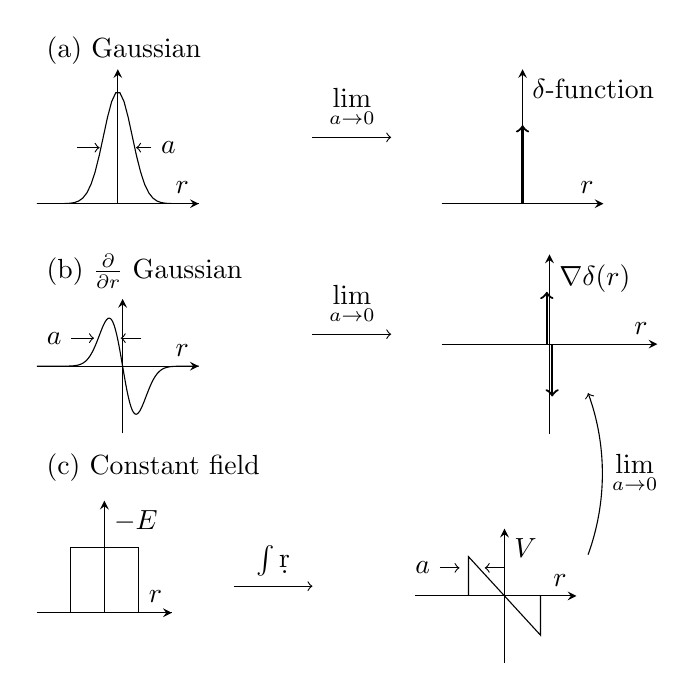
\begin{tikzpicture}

  % case (a)
  \node[anchor=west] at (0,1.8) {(a) Gaussian};

  % Gaussian
  \begin{axis}[
        xmax=4,ymax=1.2,
        xmin=-4,ymin=0,
        samples=50,
        axis lines=middle,
        ytick style={draw=none},
        xtick style={draw=none},
        yticklabels={,,},
        xticklabels={,,},
        xlabel={$r$},
        ylabel={},
        scale=0.3,
        at = {(0,-10)},
     ]
     \addplot[black] {exp(-x^2)};
     \node (a) at (axis cs:2.5,.5) {$a$};
     \draw[->] (a) -- (axis cs:.9,.5);
     \draw[->] (axis cs:-2.0,.5) -- (axis cs:-.9,.5);
  \end{axis}

  % arrow with limit
  \draw[->] (3.5,.7) -- node [midway, above] {$\lim\limits_{a\to0}$} (4.5,.7);

  % delta function
  \begin{axis}[
        xmax=4,ymax=1.2,
        xmin=-4,ymin=0,
        samples=150,
        axis lines=middle,
        ytick style={draw=none},
        xtick style={draw=none},
        yticklabels={,,},
        xticklabels={,,},
        xlabel={$r$},
        ylabel={$\delta$-function},
        scale=0.3,
        at = {(2000,-10)},
     ]
     \draw[->, thick] (axis cs:0,0) -- (axis cs:0,.7);
  \end{axis}

  % case (b)
  \node[anchor=west] at (0,-1) {(b) $\frac{\partial}{\partial r}$ Gaussian};

  % (d/dr) Gaussian
  \begin{axis}[
        xmax=4,ymax=1.2,
        xmin=-4.5,ymin=-1.2,
        samples=150,
        axis lines=middle,
        ytick style={draw=none},
        xtick style={draw=none},
        yticklabels={,,},
        xticklabels={,,},
        xlabel={$r$},
        ylabel={},
        scale=0.3,
        at = {(0,-430)},
     ]
     \addplot[black] {-2*x*exp(-x^2)};
     \node (b) at (axis cs:1.5,.5) {};
     \draw[->] (b) -- (axis cs:-.1,.5);
     \node[left] (a) at (axis cs:-2.7,.5) {$a$};
     \draw[->] (a) -- (axis cs:-1.5,.5);
  \end{axis}

  % arrow with limit
  \draw[->] (3.5,-1.8) -- node [midway, above] {$\lim\limits_{a\to0}$} (4.5,-1.8);

  % two delta functions
  \begin{axis}[
        xmax=4,ymax=1.2,
        xmin=-4,ymin=-1.2,
        samples=150,
        axis lines=middle,
        ytick style={draw=none},
        xtick style={draw=none},
        yticklabels={,,},
        xticklabels={,,},
        xlabel={$r$},
        ylabel={$\nabla\delta(r)$},
        scale=0.4,
        at = {(1500,-323)},
     ]
     \draw[->, thick] (axis cs:-.1,0) -- (axis cs:-.1,.7);
     \draw[->, thick] (axis cs:.1,0) -- (axis cs:.1,-.7);
  \end{axis}

  % case (c)
  \node[anchor=west] at (0,-3.5) {(c) Constant field};

  % constant field
  \begin{axis}[
        xmax=4,ymax=1.2,
        xmin=-4,ymin=0,
        samples=150,
        axis lines=middle,
        ytick style={draw=none},
        xtick style={draw=none},
        yticklabels={,,},
        xticklabels={,,},
        xlabel={$r$},
        ylabel={$-E$},
        scale=0.25,
        at = {(0,-450)},
     ]
     \addplot[const plot, no marks, black] coordinates {(-2,0) (-2,.7) (2,.7) (2,0) (4,0)};
  \end{axis}

  % arrow with integral
  \draw[->] (2.5,-5) -- node [midway, above] {$\int\d r$} (3.5,-5);

  % truncated linear potential
  \begin{axis}[
        xmax=4,ymax=1.2,
        xmin=-5,ymin=-1.2,
        samples=150,
        axis lines=middle,
        ytick style={draw=none},
        xtick style={draw=none},
        yticklabels={,,},
        xticklabels={,,},
        xlabel={$r$},
        ylabel={$V$},
        scale=0.3,
        at = {(2100,-840)},
     ]
     \addplot[no marks, black] coordinates {(-2,0) (-2,.7) (2,-.7) (2,0)};
     \node (b) at (axis cs:.5,.5) {};
     \draw[->] (b) -- (axis cs:-1.1,.5);
     \node[left] (a) at (axis cs:-3.6,.5) {$a$};
     \draw[->] (a) -- (axis cs:-2.5,.5);
  \end{axis}

  % arrow with limit on an arc
  \draw[->] (7,-4.6) arc (-20:20:3) node [midway,right] {$\lim\limits_{a\to0}$};

\end{tikzpicture}

    \caption[Schiff moment as electric field inside a nucleus.]{\part{a} Delta function as the limit of a Gaussian. \part{b} Gradient of a Gaussian as a representation of $\nabla\delta(r)$. \part{c} Constant field inside the nucleus gives rise to a truncated linear potential, which has a similar shape to the derivative of the Gaussian and in the appropriate limit becomes $\nabla\delta(r)$.}
   \label{graddelta}
\end{figure}

We may think of the Schiff moment as due to a constant electric field along the
direction of the nuclear spin $\hat I$ inside a nucleus of radius $R_0$. This
potential is linear in the coordinate $r$ and truncated outside of the nucleus
(i.e., at $|r|>R_0$). In the limit of a small nucleus, this will have a similar
shape (Fig.~\ref{graddelta}c) as the expression $\nabla\delta(\vec R_0)$
discussed in the preceding paragraph.

It is possible to estimate the magnitude of the Schiff moment inside a nucleus
with a dipole moment $d_\text{N}$ and a uniform spherical core of radius $R_0$.
The \gls{EDM}\ includes additive contributions from both the nucleon \gls{EDM}
s, arising from short-range interactions between quarks, and also from
longer-range $P,T$-violating interactions between valence nucleons and the core.
In fact, in some theory models, the latter contribution to the \gls{SMT}\ can be
10 to 100 times larger than that due to the nucleonic \gls{EDM}.
\cite{sushkov1984possibility} Consider models for each case:

(1) Inside the uniform charge distribution---which does not contribute to the
\gls{SMT}---there are in addition two point charges, separated by a distance
$2R_0$ along the $z$ axis. The charge asymmetry is defined with respect to the
spin axis. In the multipole expansion, the terms are grouped by the power of the
spin operator. These powers can be either even or odd with respect to time
reversal.  The $T$-odd part of the nuclear charge can thus be written as
%
\[
\rho(\vec R)=\frac{d_\text{N}}{2eZR_0}\big[
     \delta^3(\vec R-R_0\hat{\vec z})
    -\delta^3(\vec R+R_0\hat{\vec z})
\big],
\]
%
the constant factors being chosen so that $e\ex{\vec R}=d_\text{N}\hat{\vec z}$.
Evaluating the third moments in eqn~\ref{simpleSchiffMoment}, we readily see
that the magnitude of the \gls{SMT}\ is $|\vec S|=d_\text{N}R_0^2/10$.

(2) Instead of the two separated point charges, suppose the nucleus consists of
closed shells, plus a valence proton (or neutron) that carries a dipole moment
$d_\text{p}$. Further suppose that the valence nucleon is distributed uniformly
throughout the nucleus, so that the nucleus has uniformly distributed electric
polarization. It is a standard result that the charge distribution of a
uniformly polarized sphere is exactly a surface charge, with charge density
%
\[
\rho(\vec R)=\frac{d_\text{p}}{4\pi eZR_0^3/3}\delta(R_0-R)\cos\theta,
\]
which integrates to $e\ex{\vec R}=d_\text{p}\hat{\vec z}$, and the Schiff moment is
%
\begin{equation}
    \label{protonSMT}
    |\vec S|=d_\text{p}R_0^2/10.
\end{equation}
%
We have seen that the effect of this electric field at the site of the nucleus
would be to polarize the atom, and give rise to a potentially measurable energy
shift.

In each case, we saw that $|\vec S|\propto R_0^2$. Furthermore, the matrix
element proportional to the first order energy shift has a $Z^2$ dependence.
Since the nuclear radius scales as $R_0\approx R_\text{N}A^{1/3}$, where
$R_\text{N}\approx1.2\fm$ is the characteristic nuclear size
\cite[eqn~3.8]{krane1987introductory}, the overall scaling is $Z^2 A^{2/3}$. We
conclude that heavier atoms---such as thallium---are preferable for \gls{SMT}\
experiments.

\subsection{New physics in molecules}

For nuclei inside a molecule, the Schiff moment and other $P,T$-violating
effects give rise to an effective interaction of form
%
\begin{equation}
   \label{interaction}
    \H_{\text{eff}}=-\nu\hat{\vec I}\cdot\hat{\vec n},
\end{equation}
%
where $\hbar\hat{\vec I}/2$ is the nuclear spin, and $\hat{\vec n}$ is a unit
vector along the internuclear axis in the molecule (in TlF, we define this to
point towards the F nucleus). Compared to the atomic case, in a diatomic
molecule there is another inherent direction: along the internal electric field,
pointing along the internuclear axis. The interaction strength $\nu$ can then be
interpreted in terms of a molecular \gls{EDM}, proton \gls{EDM}, Schiff moment,
or other quantities.

Without an external electric field, the interaction of eqn~\ref{interaction}
fails to produce any first order effects in any given rotational state.
According to \cite{hinds1980experiment,wilkening1984search}, this is because the
Tl nuclear spin is perpendicular to the internuclear axis in an unpolarized
molecule. Stated more correctly, the rotation of the molecule averages
$\hat{\vec n}$ to zero, and the Schiff shift---proportional to the internal
molecular field---vanishes. \cite{cho1989tenfold, cho1991search} However, if we
apply an external field, the molecule becomes polarized, which destroys the
inversion symmetry and a nonzero expectation of $H_{\text{eff}}$ results.

\begin{figure}
    \def\svgwidth{\columnwidth}
    \makebox[\columnwidth][c]{%
        \footnotesize
        \input{figs/matplotlib/polarizeTlF.pdf_tex}
    }
    \caption[Polarization of TlF molecules in external field.]{Degree of
    polarization of TlF molecules in an external field. The legends give the
    labels $(J,m_J)$. Note that $J$ is not a good quantum number at high fields
    and is to be understood in an asymptotic sense. The calculation that
    produces this figure is presented in Appendix~\ref{TlF_hamiltonian_python}.}
    \label{polarizeTlF}
\end{figure}

\paragraph{Polarization}

Compared to atoms, molecules can be polarized much more readily in laboratory
fields owing to their smaller level separation (tens of GHz, or $10^{-4}\eV$,
instead of the typical atomic eV-scale spacing), making them ideal for an
\gls{EDM}\ measurement. Thus Sandars \cite{sandars1967measurability} suggested a
molecular-beam resonance experiment could be used to probe the existence of an
electric dipole moment on the proton, so long as the molecule has a heavy atom
with an unpaired proton in the nucleus.

The polarization of molecules is so effective that the first order model,
entirely suitable for atoms, no longer applies. When the coupling
$D_\text{sp}\mathcal{E}+\delta_T$ is no longer small compared to the level
separation, the states get mixed with a mixing coefficient of order unity. It is
customary to define the degree of polarization $\mathcal{P}$ of a state $\psi$
as the expectation value of the cosine of the angle $\theta$ between the
internuclear axis and the external field:
%
\begin{equation}
    \label{polarizationdefinition}
    \mathcal{P}\equiv
    \frac{\ex{\hat{d_z}}}{D_\text{sp}}
    =\ex{\cos\theta},
\end{equation}
%
where the expectation values $\ex{\cdots}$ are of course evaluated as
$\bra\psi\cdots\ket\psi$. See Fig.~\ref{polarizeTlF} for a plot of $\mathcal{P}$
in some of the lowest-lying rotational states of TlF; observe how states that
are lower in energy are easier to polarize, while some of the higher-lying
states can even be polarized against the direction of the applied field at some
field magnitudes. Despite the fact that the $J=0$ states can be polarized better
than the $J=1$, $m_J=\pm1$ ones, we prefer the latter due to their internal
magnetic field, which is nearly exactly aligned with the applied electric field.
The former states woud necessitate applying an external magnetic field,
suffering from the motional magnetic field systematic (discussed in section
\ref{section:systematics}).

As we have seen previously, a $T$-violating interaction such as the Schiff
moment inside a fully polarized molecule gives rise to a first order energy
shift $h\nu$ as in eqn~\ref{schiffnumbers}. We have also seen two simple models
of how a dipole moment $d$ inside the nucleus results in a \gls{SMT}\ of
magnitude $S=ZdR_0^2/10$. We may thus estimate the size of an effective internal
molecular electric field $\mathcal E_\text{int}^\text{eff}$ in the
fully polarized TlF molecule via the definition
%
\begin{equation}
    \label{effestimate}
    \mathcal E_\text{int}^\text{eff}\equiv\frac{h\nu}{d}
    =1.98\cdot10^6\frac{h\;\text{Hz}}{e\;\text{fm}^3}\frac{R_0^2}{10}
    \approx408~\text{kV/cm},
\end{equation}
%
where, as previously stated, $R_0\approx R_\text{N}A^{1/3}$, with the
characteristic nuclear size $R_\text{N}\approx1.2\fm$.

We emphasize that this is not the average field in the volume of the nucleus;
that field must be zero to keep the nucleus from accelerating out of the
molecule. Nor is $\mathcal E_\text{int}^\text{eff}$ to be taken as a proxy for
the simple $\sim$~GV/cm field due to the nuclear charge at a distance of order
$a_0$ from the nucleus. The numerical values in
eqn~\ref{effestimate} obtain different estimates in different papers; for
example 20~kV/cm in ref.~\cite{harrison1969experimental} and 32.3~kV/cm in
ref.~\cite{petrov2002calculation}. Trying to estimate a generalized form of the
\gls{SMT}, Flambaum and Ginges \cite{flambaum2002nuclear} found the ``analytical
calculation hopeless [for] a nucleus with an external proton in state $s_{1/2}$,
as is the case for $^{203,205}$Tl.''

\paragraph{Separated oscillatory fields}

To obtain an upper bound on $\nu$, a pair of states is chosen such that one of
the states moves up in energy due to the interaction in eqn~\ref{interaction},
and the other one down by the same amount, increasing the level separation by
$2\nu$. Upon reversal of externally applied fields, the directions of the level
shifts change and a level separation of $-2\nu$ obtains compared to the levels
in absence of the interaction. (See Fig.~1 of ref.~\cite{hinds1980experiment} or
\cite{wilkening1984search} for a diagram.) Comparing the two perturbations of
the level spacing, a $4\nu$ difference (together with its error bars) can be
quoted as the main result of molecular-beam symmetry-violation experiments.

The spacing between the levels can be measured by a \gls{NMR} technique based on
Rabi oscillations. Consider two states, $\ket p$ and $\ket q$, separated by an
energy $\hbar\omega_0$, and placed in an oscillating field $\hbar b
e^{-i\omega\tau}$.  Defining the detuning $\delta\equiv\omega_0-\omega$, the
population transfer probability is given by \cite[eqn~V.10]{ramsey1956molecular}
%
\begin{align*}
    P_{p,q}=
    \left(\frac{2b}{\Omega}\right)^2
    \sin^2
    \left(
    \frac{\Omega\tau}{2}
    \right),
    \;\text{with}\;
    \Omega=\sqrt{\delta^2+(2b)^2}.
\end{align*}
%
We see the transfer is maximised for a resonant field, $\omega=\omega_0$, and
the full width at half maximum (\FWHM) is given by $\Delta\omega=4b$. For a
resonant $\pi/2$ pulse of duration $T=\pi/2b$, the \FWHM\ will be
$\Delta\omega=2\pi/T$, and the longer the precession period $T$, the more
precisely we can determine the resonant frequency $\omega_0$.

In principle, an infinitely precise measurement could be obtained by simply
extending the length $l$ of the precession region, thus prolonging the
precession period $\tau=l/v$ for molecules of speed $v$. In practice, however,
this meets with the following problems. (1) The beam intensity $N$ decays as
$1/l^2$ in the limit where the interaction region is long compared to the
distance from the source to the start of the interaction region. Indeed, the
signal-to-noise ratio, being proportional to $\sqrt{N}/\tau$, is roughly
independent of interaction length. (2) We may want to measure the precession in
a region where the oscillating field cannot be applied. (3) It is difficult to
maintain uniform externally applied fields over an extended length.

It turns out that the oscillating field does not need to extend over the entire
length of the precession region. In Ramsey's resonance scheme, \gls{SOF} are
only applied in two small regions at the beginning and at the end of the
interaction region, each applying a $\pi/2$ pulse. The resulting \FWHM\ is about
40\%\ smaller that that obtained in a simple Rabi oscillation scheme, and the
resonances are less broadened by the non-uniformity of the fixed field.
\cite{PhysRev.78.695} One way to understand the latter point is to note that the
oscillating field driving the transitions at each end will be tuned to the
nominal resonant frequency determined by the level spacing in the region of the
\RF\ coils. If, in the region between the two coils, the residual fields cause
the level spacing to deviate from its nominal value, this should not affect the
efficacy of the coils.

The transition probability $\widetilde{P}_{p,q}$ for the \gls{SOF} scheme, here
expressed in terms of the simple Rabi oscillation probability $P_{p,q}$, is
\cite[cf.\ eqn~V.37]{ramsey1956molecular}
%
\[
    \frac{\widetilde{P}_{p,q}}
    {P_{p,q}}=4
    %\sin^2\Theta\sin^2\frac{\Omega\tau}{2}
    \left[
        \cos\frac{T\overline{\delta}-\phi}{2}\cos\frac{\Omega\tau}{2}
        -
        \frac{\delta}{\Omega}
        \sin\frac{T\overline{\delta}-\phi}{2}\sin\frac{\Omega\tau}{2}
    \right]^2
    ,
\]
%
where $\overline{\delta}\equiv\overline{\omega}_0-\omega$ is the detuning of the
oscillating field frequency $\omega$ from the level separation
$\hbar\overline{\omega}_0$, averaged over the length of the interaction region,
and $\phi$ is the phase delay between the two oscillating coils. Now $T$ is the
duration of the molecular flight through the field-free region, while $\tau$ is
the duration of each of the oscillating-field regions. Of course, as a molecule
flies through the different regions, the oscillating field is not turned off or
on instantaneously; nevertheless, the effect of the smooth turn-on if simply a
modified strength of the oscillating field, for which we compensate by directly
optimizing the field strength.

\begin{figure}
    \def\svgwidth{\columnwidth}
    \makebox[\columnwidth][c]{%
        \footnotesize
        \input{figs/matplotlib/SOF.pdf_tex}
    }
    \caption[Separated oscillatory fields vs Rabi oscillation.]{Transition
    probability as a function of detuning $\delta$, averaged over the
    effusive-source speed distribution $v^3e^{-v^2/\alpha^2}$, for a precession
    length $L=10l$. \part{a} Comparing \gls{SOF} ($\tilde
    b_\text{\gls{SOF}}=0.600$, $\phi=0$) and Rabi oscillations ($\tilde
    b_\text{Rabi}=1.200$), both with the same $L$. Notice the $\approx40$\%\
    narrower \FWHM\ for \gls{SOF}. \part{b} Detection scheme sensitive to small
    $\delta$: \gls{SOF}\ with $\phi=\pi/2$ with the same $L=10l$.}
    \label{SOFprob}
\end{figure}

Schropp \cite{schropp1988thesis} draws a parallel between the method of
\gls{SOF}, where a frequency-domain interference pattern is caused by two coils
that are separated in times, and Young's double-slit experiment, where the
distance between two slits causes a spatial interference pattern. In either
case, the linewidth is inversely proportional to the field-free separation,
whether a spatial one (double slits) or a temporal one (\gls{SOF}).

The above transition probabilities hold for the case of molecules subjected to
the specified interactions for a fixed amount of time. However, in a realistic
molecular beam there is a distribution of velocities $v$ and a corresponding
distribution of times $\tau=l/v$ the perturbations act. We first consider the
normalized probability density function corresponding to effusive beam sources,
as used in the classic paper by Ramsey et al. \cite{wilkening1984search}:
%
\begin{equation}
    \label{avgint}
    f(v)=
    \frac{2}{\alpha^4}
    v^3
    e^{-v^2/\alpha^2},
    \quad
    \alpha=\sqrt{\frac{2kT}{m}},
\end{equation}
%
which is simply a Boltzmann distribution with an extra factor of $v$ to account
for the fact that faster molecules preferentially escape from the cell. The
parameter $\alpha$ is the most probable molecular velocity, as well as a measure
of the spread of velocities.

The Rabi oscillation probability $P_{p,q}$ can thus be averaged over the chosen
distribution of molecular speeds $f(v)$ as
%
\begin{equation}
    \label{effusivef}
    \ex{P_{p,q}}\equiv
    \int\limits_0^\infty P_{p,q}\,f(v)dv
    .
\end{equation}
%
The optimal choice of the oscillation strength $b$ is directly related to the
length of the resonance region $l$ and the molecular velocity (or velocity
spread) $\alpha$, making $\pi\alpha/2l$ a convenient choice of frequency units.
Thus we put $b=\tilde b(\pi\alpha/2l)$, defining the dimensionless oscillation
strength $\tilde b$, and analogously for $\tilde\delta$ and $\tilde\Omega$. The
integral in eqn~\ref{avgint} can be expressed in terms of a Meijer $G$-function
\cite[sect~5.3]{erdelyi1953higher} as
%
\[
    \ex{P_{p,q}}=
    \frac{2\tilde b^2}{\tilde\Omega^2}
    -\frac{\pi^{5/2}\tilde b^2}{8}
    G_{0,3}^{2,0}\left(
        \frac{\pi^2\tilde\Omega^2}{16}
        \bigg|
        -1,1,-\frac{1}{2}
    \right)
\]
%
The $G$-function can be evaluated numerically; in particular, we find that
$\ex{P_{p,q}}(\tilde\delta=0)$ is maximised for $\tilde b=1.200$.

The distribution-averaged form of the \gls{SOF} probability
$\widetilde{P}_{p,q}$ can also be found in terms of special functions, but is
considerably more complicated. In addition to the length $l$ of the two
oscillating coils, there is a further dependence on the free-precession length
$L$, as well as the phase delay $\phi$ between the two coils. If the coils
oscillate in phase ($\phi=0$), the peak of the transition probability is
centered around the resonant frequency with no linear dependence on the detuning
$\delta$. Thus \gls{SOF} experiments commonly take $\phi=\pm\pi/2$ as in
ref.~\cite{ramsey1951phase}, where
%
\[
    \ex{\widetilde{P}_{p,q}}
    \approx
    0.383
    \pm(0.599+0.495L/l)\tilde\delta
    +O(\tilde\delta^2);
\]
%
the two choices of $\phi$ are depicted in Fig.~\ref{SOFprob}. The above numbers
assume $\tilde b=0.600$, which is the optimal value of $\tilde b$ for separated
oscillatory fields in the sense of maximum on-resonance transition probability
(for $\phi=0$), or maximum slope of $\ex{\widetilde{P}_{p,q}}$ around the
resonance (for $\phi=\pi/2$). We see that the slope is directly proportional to
the length of the free-precession region, as expected.

It will be noticed that there are high-slope regions in Fig.~\ref{SOFprob} for
both $\phi=0$ and $\phi=\pm\pi/2$, however for $\phi=\pm\pi/2$, the maximum
slope region appears at zero detuning. Due to a pulse-to-pulse variation in the
beam properties, the exact width of the resonance (and thus the position of the
highest-slope part of the $\phi=0$ curve) would change over time, whereas a zero
detuning always occurs in the same place despite the beam parameters, and only
the slope itself changes.

For a cryogenic buffer-gas beam source, the appropriate averaging is to be taken
over an offset-Gaussian distribution of molecular velocities:
%
\[
    \ex{\widetilde P_{p,q}}_\text{BG}\equiv
    \int\limits_{-\infty}^\infty P_{p,q}\,f_\text{BG}(v)dv
    ,\quad
    f_\text{BG}(v)=
    \frac{e^{-(v-\overline v)^2/2\alpha^2}}{\sqrt{2\pi}\alpha}
    ,
\]
%
where $\overline v$ is the average (center of mass) velocity of the molecular
beam, with a spread of velocities $\alpha$. The extended integration limits
compared with eqn~\ref{effusivef} are not significant, since the
$f_\text{BG}(v)\to0$ for $v$ far away from $\overline v$. See Fig.~\ref{SOF2}
for typical parameter values. Since the measurement is repeated for each sign of
$\phi=\pm\pi/2$, we can define the signal $S_\text{\gls{SOF}}$ as
%
\[
    S_\text{\gls{SOF}}=
    \ex{\widetilde P_{p,q}}_\text{BG}(\phi=\pi/2)
    -\ex{\widetilde P_{p,q}}_\text{BG}(\phi=-\pi/2),
\]
%
as displayed in Fig.~\ref{SOF2}a. For the parameter values in that figure, the
slope of $S_\text{\gls{SOF}}$ around zero detuning is approx.\ 0.094/Hz.

\begin{figure}
    \def\svgwidth{\textwidth}
    \parbox[c][8cm]{\textwidth}{%
        \footnotesize
        \input{figs/matplotlib/SOF2.pdf_tex}
        }
    \caption[SOF signal averaged over a Gaussian distribution.]{Buffer-gas
    \gls{SOF} signal as a function of detuning $\Delta f$ in linear units, averaged
    over a Gaussian speed distribution $\exp[{-(v-\overline v)^2/2\alpha^2}]$
    with $\overline v=200$~m/s and $\alpha=10$~m/s, for a 3~m separation between
    the oscillatory coils, and field strength $b=9.975\,\pi\alpha/2l$. Observe
    the effect of the finite coil length: $l=1$~cm (thick gray) and $l=10$~cm
    (thin black). \part{a} Difference in the averaged probabilities between
    $\phi=\pi/2$ and $\phi=-\pi/2$. \part{b} Averaged transition probability for
    $\phi=0$ (detail).}
    \label{SOF2}
\end{figure}

\paragraph{Beam sources}
\label{sect:beamsources}

The earliest molecular beams of thallium fluoride were of a thermal design,
where a mass of the solid salt is heated in a copper oven to raise the vapour
pressure. Depending on the mean free path (\mfp) of the molecules in the oven,
we can distinguish two main types of thermal sources. In \emph{effusive}
sources, the \mfp\ is comparable with the linear dimension $d$ of the hole
through which the molecules emerge from the beam source. The particles escape by
chance, and the beam properties reflect the state of the molecules in the oven.
By contrast, in \emph{jet sources}, the \mfp\ is much smaller than $d$. The beam
properties no longer reflect those of the oven molecules; instead, the local
thermal (electronic, rotational, and vibrational) is partly converted into the
center-of-mass motion of the particles. These beams are thus faster but colder.

For example, Schropp et al.\ \cite{schropp1987new,schropp1988thesis} report
having a source at temperature 380\degC\ that yields a fraction $3\times10^{-4}$
of molecules in the desired state $J=1$, $m_J=0$, out of a detected beam of
$7.5\times10^9$ molecules/second. The beam velocity can be estimated as
$v_\text{CM}=\sqrt{2kT/m}\approx230$~m/s, with a spread of order
$v_\text{CM}\sqrt{\ln2}\approx190$~m/s.

At the oven temperature of 380\degC, we expect approximately 25\%\ of molecules
to exist as a monomer, the rest being mostly dimers (TlF)$_2$. In addition to
decreasing the useful signal, dimers were twice as effective at producing
background counts with the detection technology used. However, by Le Chatelier's
principle the equilibrium of the endothermic reaction
$\text{(TlF)}_2\rightleftharpoons2\text{TlF}$ can be shifted towards the right
by an increase in temperature or a decrease in pressure. Thus the oven consists
of two stages: a lower, high-pressure section with the boiling salt, and an
uppper, lower-pressure region, separated by a constriction. As a result, the
monomer fraction may be as high as 50\%\ in the two-chamber design.

As an example of a jet source, Cho et al. \cite{cho1990thesis,cho1991search}
constructed a thermal source with an oven at 753~K that yielded
$1.25\times10^{10}$ molecules per second, of which $2.7\times 10^{-3}$ were in
the desired $J=1$ state for an estimated rotational temperature of $350\pm50$~K.
The beam velocity is given as $344\pm20$~m/s, with a spread of ($150\pm12$)~m/s,
giving a rotational temperature of $300\pm50$~K. As expected, the beam is both
colder and faster than the effusive source from ref.~\cite{schropp1987new}. The
higher pressure in a jet source might be expected to result in a lower monomer
fraction despite the higher temperature. To counteract this, the authors led the
beam from the oven through a 30~cm long nozzle, 20~K hotter than the oven. They
calculate that due to the approx.\ 100 times smaller density of TlF in the
nozzle compared to the oven, the monomer fraction is as high as 92\%.

The recent trend is towards cryogenic buffer-cooled beam sources. A non-reactive
buffer gas is flowed through a copper cell kept at a temperature $T_0$. The flow
rate $F$ of the buffer gas controls the numbre density of the buffer gas in the
cell. The species of interest is injected at a temperature much higher than
$T_0$ and thermalizes through with the buffer gas, cooling its rotational and
translational degrees of freedom to approximately $T_0$. Since the cell is at a
cryogenic temperatures, all target molecules that collide with the walls stick
to it, while others escape through an exit aperture in the cell; the ratio of
the time scales of these two processes determines the extraction efficiency of
the cell. Beam properties are largely determined by the collisions between the
target particles and the buffer gas around the exit aperture. See
\cite{hutzler2012buffer} for a review of cryogenic buffer gas beam sources.

Barry et al. \cite{barry2011bright} report on a cryogenic buffer-gas source for
strontium monofluoride, yielding some $1.2\times10^{11}$ molecules/sr/pulse that
are in the desired rovibronic state. At 140~m/s, the beam is slower than a
comparable thermal beam, while the rotational temperature is around 1~K. The
cell (internal volume 15~cm$^3$) was kept at 3~K, and the flow of helium
controlled at 5~sccm. The beam escapes from the cell through a 3~mm diameter
hole in a 0.5~mm thick copper plate. The beam source design has been adapted by
Norrgard et al.\ \cite{norrgard2017hyperfine} to produce a beam of thallium
fluoride.

In \CENTREX, we use neon as the buffer gas. Compared to helium-based sources,
neon allows the cell temperature to be higher ($\sim$20~K instead of $\sim$4~K)
for a compable beam velocity after gas expansion (but at a higher temperature).
Furthermore, neon is efficiently cryopumped by cold surfaces found in the beam
source unlike helium, for which a large-area adsorbent, such as activated
charcoal, is necessary. Neon also allows operation at higher pulse
rates, up to 50~Hz, which has not been found practical with helium
sources. \cite{hutzler2012buffer}

\subsection{The TlF molecule}

TlF is a suitable system to look for $P$ and $T$ violating interactions for a
number of reasons: a molecular beam of thallium fluoride can readily be obtained
by following the lead of a number of previously published papers; the properties
of the molecular states and transitions are available in the literature; the
species is a polar diatomic molecule, enhancing the effective electric field
acting at the site of the nuclei; the thallium nucleus being very heavy, the
Schiff moment is correspondingly relatively large; and the nucleus contains an
unpaired proton, making measurements potentially sensitive to proton \gls{EDM}\
effects. \cite{sandars1967measurability, wilkening1984search} By contrast, TlF
is not a suitable system for electron \gls{EDM}\ measurements due to the closed
shells' zero total electron spin. \cite{kozlov1995parity}

Thallium comes in two naturally occurring isotopes, 203 (29.52\% abundance) and
205 (70.48\%), while $^{19}$F is the only isotope of fluorine \cite{awic2015}.
In \CENTREX, we are only making use of the more abundant isotope $^{205}$Tl, and
only the transitions between the $v=0$ vibrational sublevels of the electronic
states $X^1\Sigma^+$ and $B^3\Pi_1$, where $X$ denotes the ground state, and $B$
is one of the excited states with a lifetime of about 99~ns
\cite{norrgard2017hyperfine}. The quantum numbers used to describe the states
usually refer to a modified Hund's case (c) basis with the additional couplings
$\vec F_1=\vec J+\vec I_1$ and $\vec F=\vec F_1+\vec I_2$, where $\vec I_1$ and
$\vec I_2$ refer to thallium and fluorine nuclear spins, respectively; both
nuclei are spin-half.

A particular rotational hyperfine level can be written in either the coupled or
decoupled basis, as follows:
%
\begin{align*}
    \ket{\psi_\text{coup.}} &=
    \ket{J,\Omega,m_J,I_1,F_1,I_2,F,m_F}
    \\
    \ket{\psi_\text{dec.}} &=
    \ket{J,\Omega,m_J}
    \ket{I_1,m_1}
    \ket{I_2,m_2},
\end{align*}
%
where $\Omega$ is the projection of J on the internuclear axis and $m_F$ is the
projection of $F$ in the laboratory frame. \cite{norrgard2017hyperfine} The
change of basis transformation between the two representations is simply a
matter of applying the definition of the Clebsch-Gordan coefficients
\cite[eqn~5.77]{brown2003rotational} twice to decouple $\vec F$, then $\vec
F_1$, into the constituent spins $\vec J$, $\vec I_1$, and $\vec I_2$.

\paragraph{Ground state}

The structure of the ground state can be described by the effective Hamiltonian
given in ref.\ \cite{wilkening1984search}:
%
\begin{equation}
   \label{TlF_hamiltonian}
\begin{aligned}
    \mathcal{H}_\text{TlF}&=\mathcal H_\text{rot}+\mathcal H_\text{S}+\mathcal H_\text{Z}+\mathcal H_\text{sr}+\mathcal H_\text{ss},\quad\text{where}\\
    \mathcal H_\text{rot}&=h B\vec J^2\\
    \mathcal H_\text{S}&=-\vec\mu_e\cdot\vec E\\
    \mathcal H_\text{Z}&=-\frac{\mu_J}{J}(\vec J\cdot\vec B)-\frac{\mu_1}{I_1}(\vec I_1\cdot\vec B)-\frac{\mu_2}{I_2}(\vec I_2\cdot\vec B)\\
    \mathcal H_\text{sr}&=c_1(\vec I_1\cdot\vec J)+c_2(\vec I_2\cdot\vec J)\\
    \mathcal H_\text{ss}&=5c_3\left(
            \frac{3(\vec I_1\cdot\vec J)(\vec I_2\cdot\vec J)
                +3(\vec I_2\cdot\vec J)(\vec I_1\cdot\vec J)-2(\vec I_1\cdot\vec I_2)\vec J^2}
            {(2J+3)(2J-1)}
        \right)
        \\
        &\mspace{40mu}+c_4(\vec I_1\cdot\vec I_2)
\end{aligned}
\end{equation}

The energy levels found by diagonalizing this Hamiltonian are illustrated in
Fig.~\ref{diagram} in the absence of electric and magnetic fields. The largest
effect is the rotational energy $\H_\text{rot}=hB\vec J^2$ with the rotational
constant of order $2B=13.4~\GHz$. More precisely, the rotational-vibrational
energy levels of a diatomic molecule are given by the so-called Dunham expansion
\cite{huber2013molecular}
%
\[
    T_{vJ}={\textstyle\sum_{lm}}Y_{lm}(v+1/2)^l[J(J+1)]^m.
\]
%
In practice, however, we find that the lowest few microwave rotational
transitions are sufficiently well described using only the rotational constant
in equilibrium position $B_\text{e}\equiv Y_{01}$ and the first term
$\alpha_\text{e}\equiv-Y_{11}$ using NIST data \cite{afeefy2011nist}, yielding
the effective constant $2B=13.33466\GHz$ for the isotope
$^{205}\mathrm{Tl}^{19}\mathrm{F}$. Note that the value $2B=13.37984\GHz$, given
in Ramsey et al.\ \cite{wilkening1984search}, only takes into account
$B_\text{e}$ and is thus not appropriate for driving microwave transitions.
%2*29.9792458*(0.223150163-0.001503850/2)

Due to a coupling of molecular rotation to the nuclear spin magnetic moments,
hyperfine levels are made non-degenerate by an interaction
$\H_\text{sr}=c_1(\vec I_1\cdot\vec J)+c_2(\vec I_2\cdot\vec J)$, with
$c_1\approx126\kHz$ and $c_2\approx18\kHz$. The next largest effect, the
spin--spin interaction, is due to two distinct effects of magnitudes
$c_3=0.070\kHz$ and $c_4=-13.30\kHz$. The $c_3$ term is due to a direct
dipole--dipole coupling between the nuclear spins. In the Hamiltonian given
above, the $c_3$ term is written in an effective form, valid for small (less
than approx.\ $20\kVcm$) electric fields when $J$ is a good quantum number. At
large $E$-field values, $J$ is no longer a good quantum number, and this
approximation cannot be used. In its stead, Brown and Carrington
\cite[eqn~4.17]{brown2003rotational} give
%
\begin{equation}
    \label{newc3}
\H_\text{ddd}=\frac{g_1g_2\mu_N^2}{4\pi\epsilon_0c^2}
\left\{
    \frac{\vec I_1\cdot\vec I_2}{R^3}
    -\frac{3(\vec I_1\cdot\vec R)(\vec I_2\cdot\vec R)}{R^5}
\right\},
\end{equation}
%
where $g_{1,2}$ are the nuclear $g$-factors and $\vec R=R\hat{\vec n}$ is the
internuclear displacement vector. The interaction is proportional to a spherical
rank-2 tensor $T^2(\vec I_1,\vec I_2)$ as per eqn~1.34 in
ref.~\cite{brown2003rotational}.

At first glance, the more general form of the $c_3$ term does not change the
eigenenergies significantly. However, the slope of the \gls{NMR} resonance frequency
as a function of the applied field is a factor of $\approx2$ greater when using
eqn~\ref{newc3}, as will be seen in Fig.~\ref{Cslope}, reproducing the result
41~mHz/(V/cm) reported at 20~kV/cm in Ramsey et al.\ \cite{wilkening1984search},
while the form of the Hamiltonian as given in that paper gives only
20.2~mHz/(V/cm). The later Hinds et al.\ paper \cite{cho1991search,
cho1990thesis} seems to have copied the slope from Ramsey, claiming it holds at
29.5~kV/cm, where the correct slope (as per eqn~\ref{newc3}) would be
31.5~mHz/(V/cm).

The $c_4$ term, also known as the scalar- or $J$-coupling term, arises through a
mechanism involving the transmission of nuclear spin orientation through the
intervening electrons \cite{brown2003rotational}. It is distinguished from the
tensor interaction in that it does not depend on the angle between the nuclear
directions and the internuclear axis $\vec R$. While molecular rotation averages
the $c_3$ term to zero in the $J=0$ state, the $c_4$ term survives
\cite[sect.~7.7]{budker2004atomic}. In spherical tensor form, the interaction is
proportional to $T^1(\vec I_1)\cdot T^1(\vec I_2)$.

\begin{figure}
    \centering
        % for axis breaks
    \usetikzlibrary{decorations.markings}
    \def\MarkLt{4pt}
    \def\MarkSep{2pt}
    \tikzset{
      TwoMarks/.style={
        postaction={decorate,
          decoration={
            markings,
            mark=at position #1 with
              {
                  \begin{scope}[xslant=0.2]
                  \draw[line width=\MarkSep,white,-] (0pt,-\MarkLt) -- (0pt,\MarkLt) ;
                  \draw[-] (-0.5*\MarkSep,-\MarkLt) -- (-0.5*\MarkSep,\MarkLt) ;
                  \draw[-] (0.5*\MarkSep,-\MarkLt) -- (0.5*\MarkSep,\MarkLt) ;
                  \end{scope}
              }
           }
        }
      },
      TwoMarks/.default={0.5},
    }

\begin{tikzpicture}[scale=5]

   % length of energy level diagram lines
   \def\len{.05}

   % x-position and length and x-offset of the y-axis labels
   \def\pos{-18}
   \def\lenmark{.025}
   \def\xoffset{.18}

   % x coordinates for m = -2, ... 2
   \def\xa{-4.5*\len}
   \def\xb{-2.5*\len}
   \def\xc{-0.5*\len}
   \def\xd{+1.5*\len}
   \def\xe{+3.5*\len}
   \def\xf{-6.5*\len}
   \def\xg{+5.5*\len}

   % y offset for J = 1, 2
   \def\yA{.6}
   \def\yB{\yA+.7}

   % axis
   \draw[->,TwoMarks=0.2,TwoMarks=0.6] (\xf-\len-\xoffset, -.1)
      -- (\xf-\len-\xoffset,\yB+.25) node[above] {$E$ [kHz]};

   % brace position
   \def\bracePos{\xg+3*\len}

   % J=0 labels
   \draw [decorate,decoration={brace,amplitude=5pt,mirror,raise=4pt},yshift=0pt]
      (\bracePos,-.08) -- node (midJ0) {} (\bracePos,.08) node [black,midway,anchor=west,xshift=25] (nodeJ0) {$J=0$};
   \draw (\xf-\len-0.5*\lenmark-\xoffset, -.003325) node[anchor=east,below,xshift=\pos]
      {$-3.325$} -- (\xf-\len+0.5*\lenmark-\xoffset,-.003325) node[right,below,xshift=-\pos] {$F=1$};
   \draw (\xf-\len-0.5*\lenmark-\xoffset, .009975) node[anchor=east,above,xshift=\pos]
      {9.975} -- (\xf-\len+0.5*\lenmark-\xoffset,.009975) node[right,above,xshift=-\pos] {$F=0$};

   % J=0 lines
   \draw (\xc, -0.003325) -- (\xc+\len, -0.003325);
   \draw (\xb, -0.003325) -- (\xb+\len, -0.003325);
   \draw (\xd, -0.003325) -- (\xd+\len, -0.003325);
   \draw (\xc, 0.009975) -- (\xc+\len, 0.009975);

   % J=1 labels
   \draw [decorate,decoration={brace,amplitude=10pt,mirror,raise=4pt},yshift=0pt]
      (\bracePos,\yA-.2) -- node (midJ1) {} (\bracePos,\yA+.1) node [black,midway,anchor=west,xshift=25] (nodeJ1) {$J=1$};
   \draw (\xf-\len-0.5*\lenmark-\xoffset, \yA-.143745) node[anchor=east,below,xshift=\pos] {$-143.745$} --
      (\xf-\len+0.5*\lenmark-\xoffset,\yA-.143745) node[right,below,xshift=-\pos] {$F=0$};
   \draw (\xf-\len-0.5*\lenmark-\xoffset, \yA-.121506) node[anchor=east,above,xshift=\pos] {$-121.506$} --
      (\xf-\len+0.5*\lenmark-\xoffset,\yA-.121506) node[right,above,xshift=-\pos] {$F=1$};
   \draw (\xf-\len-0.5*\lenmark-\xoffset, \yA+.054446) node[anchor=east,below,xshift=\pos] {54.446} --
      (\xf-\len+0.5*\lenmark-\xoffset,\yA+.054446) node[right,below,xshift=-\pos] {$F=1$};
   \draw (\xf-\len-0.5*\lenmark-\xoffset, \yA+.068985) node[anchor=east,above,xshift=\pos] {68.985} --
      (\xf-\len+0.5*\lenmark-\xoffset,\yA+.068985) node[right,above,xshift=-\pos] {$F=2$};

   % J=1 lines
   \draw (\xc, \yA-.143745) -- (\xc+\len, \yA-.143745);
   \draw (\xc, \yA-.121506) -- (\xc+\len, \yA-.121506);
   \draw (\xb, \yA-.121506) -- (\xb+\len, \yA-.121506);
   \draw (\xd, \yA-.121506) -- (\xd+\len, \yA-.121506);
   \draw (\xc, \yA+.054446) -- (\xc+\len, \yA+.054446);
   \draw (\xb, \yA+.054446) -- (\xb+\len, \yA+.054446);
   \draw (\xd, \yA+.054446) -- (\xd+\len, \yA+.054446);
   \draw (\xc, \yA+.068985) -- (\xc+\len, \yA+.068985);
   \draw (\xb, \yA+.068985) -- (\xb+\len, \yA+.068985);
   \draw (\xd, \yA+.068985) -- (\xd+\len, \yA+.068985);
   \draw (\xa, \yA+.068985) -- (\xa+\len, \yA+.068985);
   \draw (\xe, \yA+.068985) -- (\xe+\len, \yA+.068985);

   % J=2 labels
   \draw [decorate,decoration={brace,amplitude=10pt,mirror,raise=4pt},yshift=0pt]
      (\bracePos,\yB-.27) -- node (midJ2) {} (\bracePos,\yB+.18) node [black,midway,anchor=west,xshift=25] (nodeJ2) {$J=2$};
   \draw (\xf-\len-0.5*\lenmark-\xoffset, \yB-.217455)
   node[anchor=east,left,yshift=-5] {$-217.455$}
      -- (\xf-\len+0.5*\lenmark-\xoffset,\yB-.217455) node[right,below,xshift=-\pos] {$F=1$};
   \draw (\xf-\len-0.5*\lenmark-\xoffset, \yB-.172936)
   node[anchor=east,left,yshift=5] {$-172.936$}
      -- (\xf-\len+0.5*\lenmark-\xoffset,\yB-.172936) node[right,above,xshift=-\pos] {$F=2$};
   \draw (\xf-\len-0.5*\lenmark-\xoffset, \yB+.105876)
   node[anchor=east,left,yshift=-5] {105.876}
      -- (\xf-\len+0.5*\lenmark-\xoffset,\yB+.105876) node[right,below,xshift=-\pos] {$F=2$};
   \draw (\xf-\len-0.5*\lenmark-\xoffset, \yB+.141095)
   node[anchor=east,left,yshift=5] {141.095}
      -- (\xf-\len+0.5*\lenmark-\xoffset,\yB+.141095) node[right,above,xshift=-\pos] {$F=3$};

   % J=2 lines
   \draw (\xc, \yB-.217455) -- (\xc+\len, \yB-.217455);
   \draw (\xb, \yB-.217455) -- (\xb+\len, \yB-.217455);
   \draw (\xd, \yB-.217455) -- (\xd+\len, \yB-.217455);
   \draw (\xc, \yB-.172936) -- (\xc+\len, \yB-.172936);
   \draw (\xb, \yB-.172936) -- (\xb+\len, \yB-.172936);
   \draw (\xd, \yB-.172936) -- (\xd+\len, \yB-.172936);
   \draw (\xa, \yB-.172936) -- (\xa+\len, \yB-.172936);
   \draw (\xe, \yB-.172936) -- (\xe+\len, \yB-.172936);
   \draw (\xc, \yB+.105876) -- (\xc+\len, \yB+.105876);
   \draw (\xb, \yB+.105876) -- (\xb+\len, \yB+.105876);
   \draw (\xd, \yB+.105876) -- (\xd+\len, \yB+.105876);
   \draw (\xa, \yB+.105876) -- (\xa+\len, \yB+.105876);
   \draw (\xe, \yB+.105876) -- (\xe+\len, \yB+.105876);
   \draw (\xc, \yB+.141095) -- (\xc+\len, \yB+.141095);
   \draw (\xb, \yB+.141095) -- (\xb+\len, \yB+.141095);
   \draw (\xd, \yB+.141095) -- (\xd+\len, \yB+.141095);
   \draw (\xa, \yB+.141095) -- (\xa+\len, \yB+.141095);
   \draw (\xe, \yB+.141095) -- (\xe+\len, \yB+.141095);
   \draw (\xf, \yB+.141095) -- (\xf+\len, \yB+.141095);
   \draw (\xg, \yB+.141095) -- (\xg+\len, \yB+.141095);

   % microwave energies
   \draw[Latex-Latex] (nodeJ0) -- node[above,sloped,rotate=180] {13.4 GHz} (nodeJ1);
   \draw[Latex-Latex] (nodeJ1) -- node[above,sloped] {26.8 GHz} (nodeJ2);

   % approximate F1 labels
   \def\FposX{-5}
   \def\FposY{15}
   \def\FposYY{22}
   \node[xshift=\FposX] at (midJ0) {\nicefrac{1}{2}};
   \node[xshift=\FposX,yshift=-\FposY] at (midJ1) {\nicefrac{1}{2}};
   \node[xshift=\FposX, yshift=\FposY] at (midJ1) {\nicefrac{3}{2}};
   \node[xshift=\FposX,yshift=-\FposYY] at (midJ2) {\nicefrac{3}{2}};
   \node[xshift=\FposX, yshift=\FposYY] at (midJ2) {\nicefrac{5}{2}};
   \node[xshift=\FposX, yshift=40] at (midJ2) {$F_1$};

\end{tikzpicture}


    \caption[Rotational spectrum of TlF.]{First three rotational levels in the
    TlF ground state $X^1\Sigma^+$ zero-field energy levels. Rotational energies
    $BJ(J+1)$ are subtracted from the energies indicated on the axis. Note the
    $(2F+1)$-fold degeneracy, corresponding to the quantum numbers
    $m_F=-F,\dots,0,\dots,F$. The numbers left of the braces are the $F_1$
    labels.}
    \label{diagram}
\end{figure}

For most of the terms in the effective Hamiltonian, the matrix elements are most
readily calculated in the decoupled basis, where the operators $\vec J^2$,
$J_z$, $I_{1z}$, $I_{2z}$ are diagonal. Most of the other operators can be
written in terms of the appropriate ladder operators $J_\pm$
\cite[eqns~3.5.39--40]{sakurai2011modern}
%
\begin{equation}
    \label{ladder}
    J_\pm\ket{J,m}=\sqrt{(J\mp m)(j\pm m+1)}\ket{J,m\pm1},
\end{equation}
%
and similarly for $I_{1\pm}$, $I_{2\pm}$ acting on the $\ket{I_1,m_1}$ and
$\ket{I_2,m_2}$ subspaces. For instance, $J_x=(J_++J_-)/2$ and
$J_y=(J_+-J_-)/2i$. The dot product of two angular momentum operators can be
written in terms of the ladder operators as
%
\begin{equation}
    \label{dotproductlabel}
    \vec A\cdot\vec B=A_zB_z+\frac{1}{2}\left(
    A_+B_-+A_-B_+
    \right).
\end{equation}
%
Equations \ref{ladder} and \ref{dotproductlabel}, together with the fact the
basis states with dissimilar labels are orthogonal, allow us to find the matrix
elements between arbitrary basis states for all terms in the Hamiltonian except
for the Start effect, to which we turn now.

The Stark Hamiltonian can be expressed explicitly in the components of the
molecular electric dipole moment and the lab-frame electric field:
%
\[
    \mathcal H_\text{s}
    =\mu_{e}\sqrt{\frac{2\pi}{3}}\begin{pmatrix}
        Y_1^{-1}-Y_1^1\\
        i(Y_1^{-1}+Y_1^1)\\
    \sqrt2Y_1^0\end{pmatrix}
    \cdot
    \begin{pmatrix}
        E_x\\E_y\\E_z
    \end{pmatrix},
\]
%
with the matrix elements written in terms of the Clebsch-Gordan coefficients
$\braket{j_1m_1j_2m_2}{jm}$ \begin{gather*}
    \langle J',m_J'|Y_1^M||J,m_J\rangle
    =\sqrt{\frac{3}{2\pi}}W_M,\quad\text{where}\\
    W_M=(-1)^{M}
    \sqrt{\frac{2 J' + 1}{2(2 J + 1)}}
    \langle J' \, 0 \, 1 \, 0 | J \, 0 \rangle
    \langle J' \, m_J' \, 1 \, -M | J \, m_J \rangle.
\end{gather*}
%
For $M=0$, the expression is nonzero only for $m_J'=m_J$:
%
\[
    W_0=
    \begin{dcases*}
        \sqrt{\frac{(J-m_J)(J+m_J)}{8J^2-2}}&\quad for $J'=J-1$\\
        \sqrt{\frac{(J-m_J+1)(J+m_J+1)}{6+8J(J+2)}}&\quad for $J'=J+1$
    \end{dcases*}
\]
%
For $M=\pm1$, we need $m_J'=m_J\pm1$:
%
\[
    W_{\pm1}=
    \begin{dcases*}
        -\frac{1}{2}
        \sqrt{\frac{(J\mp m_J)(J-1\mp m_J)}{4J^2-1}}&\quad\text{for $J'=J-1$}\\
        \frac{1}{2}
        \sqrt{\frac{(J+1\pm m_J)(J+2\pm m_J)}{3+4J(J+2)}}&\quad\text{for $J'=J+1$}
    \end{dcases*}
\]

Since the direction of motion of electrons in the atom does not change the
electric dipole moment, time reversal is a symmetry of the Stark effect.
\cite{gottfried2013quantum} It can be shown that there exist pairs of states of
opposite $m_J$ with identical matrix elements of the Stark operator $S_z$
(identical polarizabilities to first order). \cite{angel1968hyperfine}
Considering the $M=0$ expression above, corresponding to the $z$-direction of
the dipole moment, we see the $\sgn(m_J)$ dependence is gone.

We can make use of the expressions for the Stark effect matrix elements in two
other contexts. To calculate the degree of molecular polarization
(eqn~\ref{polarizationdefinition}), all it takes is the find the expectation
value of the $z$-component of the Stark Hamiltonian in an eigenstate at
particular field value, divided by $\mu_e=4.2~\text{Debye}$. The other
application is to find the matrix element of the alternative $c_3$ term
(eqn~\ref{newc3}), where the dot products $\vec I_i\cdot\vec R$ can be found in
spherical tensor notation as
%
\[
    \vec I_i\cdot\vec R
    =
    \sqrt2I_{i,0}W_0+
    \left(I_{i,1}W_{-1}-I_{i,-1}W_1\right).
\]

\paragraph{Excited state}

While the nuclear magnetic resonance occurs entirely within the $X^1\Sigma^+$
ground state, the structure of the excited state $B^3\Pi_1$ is nevertheless
important for the state preparation and readout, which we implement using
$X\leftrightarrow B$ transitions. In the following, we will present
$\Omega$-doubling in the excited state, transition nomenclature, and optical
cycling.

States $\ket{J,\Omega,m_J,I_1,F_1,I_2,F,m_F}$ are not eigenstates of parity. The
appropriate combinations of these states with a definite parity can be written
as the $\Omega$-doublets
%
\begin{equation}
    \label{doublets}
    \ket{\Omega,\pm}
    =
    \frac{1}{\sqrt2}
    \left[
       \ket{\Omega}
       \pm(-1)^{J+1}
       \ket{-\Omega}
    \right],
\end{equation}
%
with all the other quantum numbers being implied. (Note that this is not
necessary in the ground state, where $\Omega=0$.) Thus for each $J$, there is a
pair of nearly degenerate states of opposite values of parity $\pm(-1)^{J+1}$,
but the ordering of these states alternates with $J$. To avoid the alternation,
integer-$J$ states with parity $-(-1)^{J+1}$ are conventionally designated
$e$-states, and those with $(-1)^{J+1}$ are called $f$-states.
\cite[sect.~6.9.4]{brown2003rotational}

According to accepted terminology, a transition is said to belong to the $P$,
$Q$, or $R$ branches if the quantum number $J$ changes by $-1$, 0, or $+1$,
respectively. \cite[sect.~10.2]{bransden1990physics} Furthermore, we append the
$J$ number of the original state, and the $F$ of the target state. For instance,
a $P2$ $F1$ line starts in a $J=2$ state, changes $J$ by $-1$, and ends up in a
state with $F'=1$. \label{P2F1}

Despite the limited ability to collect and detect photons from fluorescing
molecules, our detection scheme could in principle detect $\approx100$\% of the
molecules through optical cycling. A laser excites the $X\to B$ transition,
causing photons in the decay back down to $X$. If the molecule ended up in the
same sublevel in $X$, the same laser can re-excite it back to $B$.
\cite{hunter2012prospects}

However, due to the large number of degrees of freedom in molecules, optical
cycling can be difficult to achieve in molecules. It turns out that in TlF,
there exists sufficiently closed transitions to allow $\sim100$ cycles before
the molecule gets lost in inaccessible dark states (see
ref.~\cite{norrgard2017hyperfine} for some possible candidates). The number of
dark states is potentially very large since the hyperfine structure (\hfs) of
the ground state is unresolved.

\paragraph{Branching ratios}

The strength of the transitions between various hyperfine states is a function
of the matrix elements of the dipole operator $\vec d$ between the states, which
we now proceed to evaluate. Working in the basis
$\ket{J,\Omega,m_J,I_1,F_1,I_2,F,m_F}$, with $I_1=I_2=\nicefrac{1}{2}$, use the
Wigner-Eckart theorem \cite[eqn~5.172]{brown2003rotational}
%
\begin{equation}
    \label{wignereckart}
    \bra{j,m}\tens T_p^k(\vec A)\ket{j',m'}=(-1)^{j-m}
    \ThreeJ{j}{k}{j'}{-m}{p}{m'}
    \bra{j}|\tens T^k(\vec A)|\ket{j'}
\end{equation}
%
to take the $m_F$ dependence out of the matrix element:
%
\begin{align}
    \label{useWE1}
    \bra{F,&m_F,\ldots}\tens T_p^1(\vec d)\ket{F',m_F',\ldots}
    \\&=\nonumber
    (-1)^{F-m_F}\ThreeJ{F}{1}{F'}{-m_F}{p}{m_F'}
    \bra{F,\ldots}|\tens T^1(\vec d)|\ket{F',\ldots},
\end{align}
%
Space and spin commute ($[\vec r,\vec I_1]=[\vec r,\vec I_2]=0$), whereas $[\vec
r,\vec J]\ne0$. Thus, $\vec I_1,\vec I_2$ are `spectator' spins, i.e., the
dipole operator $d_p$ acts only on a part of the coupled scheme. In this case,
we can apply the `spectator theorem' \cite[eqn~5.174]{brown2003rotational}
%
\begin{equation}
    \label{spectatortheorem}
\begin{aligned}
    \bra{j_1,j_2,&j}|\tens T^{k_1}(\vec A_1)|\ket{j_1',j_2',j'}
    =
    \delta_{j_2,j_2'}(-1)^{j'+j_1+k_1+j_2}\\
    &\sqrt{(2j+1)(2j'+1)}
    \SixJ{j_1'}{j'}{j_2}{j}{j_1}{k_1}
    \bra{j_1}|\tens T^{k_1}(\vec A_1)|\ket{j_1'},
\end{aligned}
\end{equation}
%
so that $j_2$ drops out of the reduced matrix element. (Note: do not use
eqn~5.136 in \cite{brown2003rotational} due to a typo in the $6j$-symbol.) We
can use that to break up the $\vec F=\vec F_1+\vec I_2$ coupling:
%
\begin{align}
    \label{useST1}
    \bra{F&,F_1,I_2\ldots}|\tens T^1(\vec d)|\ket{F',F_1',I_2',\ldots}
    =(-1)^{F'+F_1+1+\nicefrac{1}{2}}\\\nonumber
    &\sqrt{(2F+1)(2F'+1)}
    \SixJ{F_1'}{F'}{1/2}{F}{F_1}{1}
    \bra{F_1,\ldots}|\tens T^1(\vec d)|\ket{F_1',\ldots}.
\end{align}
%
We can repeat this procedure on $\vec F_1=\vec J+\vec I_1$, taking $\vec I_1$ to
be the spectator spin:
%
\begin{align}
    \label{useST2}
    \bra{F_1&,J,I_1\ldots}|\tens T^1(\vec d)|\ket{F_1',J',I_1',\ldots}
    =(-1)^{F_1'+J+1+\nicefrac{1}{2}}\\\nonumber
    &\sqrt{(2F_1+1)(2F_1'+1)}
    \SixJ{J'}{F_1'}{1/2}{F_1}{J}{1}
    \bra{J,\ldots}|\tens T^1(\vec d)|\ket{J',\ldots}.
\end{align}
%
In order to have an expression for the non-reduced matrix element, we can use
Wigner-Eckart in reverse:
%
\begin{equation}
    \label{reverseWE}
\begin{aligned}
    \bra{J,&\ldots}|\tens T^1(\vec d)|\ket{J',\ldots}
    =
    \frac{\bra{J,m_J,\ldots}\tens T_p^1(\vec d)\ket{J',m_J',\ldots}}
         {(-1)^{J-m_J}\ThreeJ{J}{1}{J'}{-m_J}{p}{m_J'}}
\end{aligned}
\end{equation}

Note that the dipole operator $\vec d=-e\vec r$ is defined in the molecule-fixed
frame. To transform from the lab frame (indices $p$) to the molecule frame
(indices $q$), we can use the relation \cite[eqn~5.182]{brown2003rotational}
%
\[
    \tens T_p^k(\vec A)
    =
    \sum\limits_q\mathcal D_{pq}^{(k)}(\omega)^*
    \tens T_q^k(\vec A),
\]
%
where $\mathcal D_{pq}^{(k)}$ are the Wigner rotation matrices as a function of
angular coordinates $\omega$. We can use this to rewrite the last matrix element
above as follows:
%
\begin{align*}
    \bra{J,m_J,&\ldots}\tens T_p^1(\vec d)\ket{J',m_J',\ldots}
    \\=
    &\bra{J,m_J,\ldots}\sum_q\mathcal D_{pq}^{(1)}\tens T_p^1(\vec d)\ket{J',m_J',\ldots}
\end{align*}
%
The operator $\tens T_q^1(\vec d)$ acts in molecule-fixed frame, in which there
is no molecular rotation, so it cannot act on the mechanical rotation part of
the $J$ angular momentum. In does, however, act on the $\vec \Omega$ part,
allowing us to split the above into
%
\begin{align*}
    \sum_q
    \bra{J,m_J,\Omega}\mathcal D_{pq}^{(1)}\ket{J',m_J',\Omega'}
    \underbrace{
        \bra{\Omega}\tens T^1_q(\vec d)\ket{\Omega'}
    }_{\delta_{q,\Omega-\Omega'}\ex{\vec d}}.
\end{align*}
%
The second factor, including the $\delta_{q,\Omega-\Omega'}$, in the expression
is the same for all $X$--$B$ transitions. For the first one, we can use the
formula \cite[eqn~5.184]{brown2003rotational}
%
\begin{align*}
    \bra{J,\Omega,&m}\mathcal D_{pq}^{(k)}(\omega)^*\ket{J',\Omega',m'}
    =
    (-1)^{m-\Omega}\\
    &\sqrt{(2J+1)(2J'+1)}
    \ThreeJ{J}{k}{J'}{-m}{p}{m'}
    \ThreeJ{J}{k}{J'}{-\Omega}{q}{\Omega'}
\end{align*}
%
with $q$ set to $\Omega-\Omega'$:
\begin{align}
    \label{userotation}
        \bra{J&,m_J,\Omega}\tens T_p^1(\vec d)\ket{J',m_J',\Omega'}
        =\ex{\vec d}(-1)^{m_J-\Omega}\\\nonumber
        &\sqrt{(2J+1)(2J'+1)}
        \ThreeJ{J}{1}{J'}{-m_J}{p}{m_J'}
        \ThreeJ{J}{1}{J'}{-\Omega}{\Omega-\Omega'}{\Omega'}.
\end{align}

Finally, it remains to collect together all the factors from equations
\ref{useWE1}, \ref{useST1}--\ref{userotation}. Rearranged for readability, we
have:
%
\begin{equation}
    \label{finalME}
\begin{aligned}
    \bra{F,m_F,&\ldots}\tens T_p^1(\vec d)\ket{F',m_F',\ldots}=
    \\&\ex{\vec d}
    (-1)^{3+F-\Omega+F_1-m_F+F'+F_1'}
    \big[{(2J+1)(2J'+1)}\\
    &\mbox{}\hspace{5ex}{(2F_1+1)(2F_1'+1)}{(2F+1)(2F'+1)}\big]^{1/2}\\
    &\SixJ{J'}{F_1'}{1/2}{F_1}{J}{1}
    \SixJ{F_1'}{F'}{1/2}{F}{F_1}{1}\\
    &\ThreeJ{J}{1}{J'}{-\Omega}{\Omega-\Omega'}{\Omega'}
    \ThreeJ{F}{1}{F'}{-m_F}{p}{m_F'}.
\end{aligned}
\end{equation}
%
As mentioned above eqn~\ref{doublets}, the decoupled basis states are not parity
eigenstates in the excited states. Thus, the appropriate matrix elements to use
are the symmetrized combinations
%
\begin{equation}
    \label{symmetrizedME}
    \frac{1}{\sqrt2}
    \big[
        \bra{\Omega}\tens T_p^1(\vec d)\ket{\Omega'}
        \pm(-1)^{J+1}
        \bra{\Omega}\tens T_p^1(\vec d)\ket{-\Omega'}
    \big],
\end{equation}
%
emphasizing again that the doublets only occur in the excited state, where
$\Omega\ne0$. Furthermore, in the excited state, energy eigenstates contain an
admixture of multiple different $\ket{J,F_1,F}$ basis states as detailed in
Table IV of ref.~\cite{norrgard2017hyperfine}; these must be taken into account
for an accurate calculation of physical matrix elements.

Appropriately normalized, eqns~\ref{finalME} and \ref{symmetrizedME} yield the
branching ratios $b_\text{e$\to$g}$ from a given sublevel $\ket{\text{e}}$ in
the excited state to a sublevel $\ket{\text{g}}$ in the ground state. The
squared magnitude of the matrix element needs to be divided by the sum over all
possible final (ground) states from the given initial (excited) state:
%
\begin{equation}
    \label{branchingratios}
    b_\text{e$\to$g}\equiv
    \frac{\sum_p|\bra{\text{e}}\tens T_p^1(\vec d)\ket{\text{g}}|^2}
         {\sum\limits_{\ket{\text{g}}}\sum_p|\bra{\text{e}}\tens T_p^1(\vec d)\ket{\text{g}}|^2},
\end{equation}
%
explicitly writing out the sum over polarizations $p$. This allows us to
immediately calculate branching ratios between pure-parity states given the
quantum numbers of each state; see Appendix~B in ref.~\cite{wenz2021thesis} for
explicit numbers.

\subsection{Previous experiments}

The first $P,T$-violation experiment using a molecular beam of thallium fluoride
was done in Oxford in 1969 \cite{harrison1969experimental}, the result being
reported as $\nu=0.08\pm0.11\Hz$, or, in terms of proton \gls{EDM}, as
$|d_\text{p}|=(7\pm9)\times10^{-21}e\cm$. They employed the triple resonance
scheme: first, $J=1$ molecules were transferred from $m_J=0$ to $m_J=\pm1$. The
second resonance which changed the Tl nuclear spin projection from $\pm1/2$ to
$\mp1/2$ is not directly observable; however, after the molecules are
transferred back to $m_J=0$, the amount of the non-observable spin flips can be
estimated and related to the desired frequency shifts $4\nu$.

About a decade later, Hinds and Sandars \cite{hinds1980experiment} reported a
similar experiment giving the null result of $\nu=11\pm42\mHz$ or
$|d_\text{p}|=(1.8\pm7)\times10^{-21}e\cm$. Looking for $P$ and $T$ violating
interactions in $^{205}$TlF, they tried to measure shifts of the resonant
frequency which depends on the relative directions of externally applied
parallel electric and magnetic fields. The experiment used a beam of TlF
produced by vapors effusing from a hot oven through a state-selecting region
that approximately transmits only molecules with $J=1$, $m_J=-1$,
$m_\text{Tl}=+\nicefrac{1}{2}$, $m_\text{F}=-\nicefrac{1}{2}$. In the
interaction region, separated oscillating magnetic fields induce some molecules
to flip the Tl spin to $m_\text{Tl}=-\nicefrac{1}{2}$. Finally, a second state
selector transmits only the molecules without the spin flip, and the final beam
intensity, as measured by a hot-wire surface ionization detector, is a sensitive
measure of the shift in the resonance given that the 10~m separation of the
oscillating coils results in a 20~Hz linewidth. However, the experiment gave an
accuracy comparable to the experiment in \cite{harrison1969experimental} because
of an unexpectedly large reduction of the resonance signal and high background
rate.

\begin{table*}
    %\small
    \makebox[\textwidth][c]{%
        \begin{tabu} to \textwidth {@{} cccc r@{$\,\pm\,$}l@{$\,\cdot\;10$}l cc @{}}
            \toprule
            Species & Type          & $E_\text{int}$ & $B_\text{int}$ & \multicolumn{3}{c}{$d$}               & Year & Ref. \\
                    &               & [kV/cm]        & [gauss]        & \multicolumn{3}{c}{[$e\cm$]} & \\\midrule
            \multicolumn{4}{@{}l}{\textit{Proton \gls{EDM}:}}\\
            TlF     & effusive beam & 80             & 26             & 7      & 9    & $^{-21}$       & 1969 & \cite{harrison1969experimental} \\
            TlF     & effusive beam & 26             & $<5\ee{-5}$    & 1.8    & 7    & $^{-21}$       & 1980 & \cite{hinds1980experiment} \\
            TlF     & effusive beam & 20.0           & $<2\ee{-3}$    & 1.3    & 2.0  & $^{-21}$       & 1984 & \cite{wilkening1984search} \\
            TlF     & jet source    & 29.5           & $<5\ee{-4}$    & 3.7    & 6.3  & $^{-23}$       & 1991 & \cite{cho1991search} \\
            \\\multicolumn{4}{@{}l}{\textit{Electron \gls{EDM}:}}\\
            Tl      & effusive beam & 50             & 1              & 6      & 12   & $^{-24}$       & 1970 & \cite{gould1970search} \\
            Tl      & effusive beam & 107            & 0.42           & 1.8    & 1.2  & $^{-26}$       & 1994 & \cite{commins1994improved} \\
            Tl      & effusive beam & 123            & 0.38           & 6.9    & 7.4  & $^{-28}$       & 2002 & \cite{regan2002new} \\
            \\\multicolumn{4}{@{}l}{\textit{Neutron \gls{EDM}:}}\\
            n       & neutron beam  & 71.6           & 250            & $-0.1$ & 2.4  & $^{-20}$       & 1957 & \cite{smith1957experimental} \\
            n       & neutron beam  & 140            & 9              & $-3$   & 8    & $^{-23}$       & 1968 & \cite{dress1968upper} \\
            n       & neutron trap  & 10             & 0.01           & 0.2    & 2.2  & $^{-26}$       & 2006 & \cite{baker2006improved} \\
            Hg      & vapour cell   & 6 \&\ 10       & 0.01           & 4.8    & 9.3  & $^{-27}$       & 2016 & \cite{graner2016reduced} \\
            n       & neutron trap  & 11             & 0.01           & 0.0    & 1.3  & $^{-26}$       & 2020 & \cite{abel2020measurement} \\
            \bottomrule
        \end{tabu}}
        \caption[Parameters of previous experiments.]{Summary of results and
        experimental parameters of some of the previous related experiments.
        $E_\text{int}$ and $B_\text{int}$ refer to the applied
        interaction-region electric and magnetic fields (and \emph{not} fields
        internal to the molecule).}
        \label{previouswork}
\end{table*}

Using a similar setup, Wilkening, Ramsey, and Larson \cite{wilkening1984search}
reduced the error bars to $\nu=8\pm21\mHz$ or
$|d_\text{p}|=(1.3\pm2.0)\times10^{-21}e\cm$. In their experiment, the thermal
beam of TlF passes through an electrostatic quadrupole field that focuses the
$J=1$, $m_J=0$ state, leaving the others unselected. Thereafter, a `subsidiary
resonance' region transfers the molecules into the state $m_J=-1$,
$m_\text{Tl}=-\nicefrac{1}{2}$, $m_\text{F}=-\nicefrac{1}{2}$. However, instead
of using oscillating fields to do so, it relies on adiabatic transitions that
conveniently happen to transfer population into the desired state. As was the
case in the preceding experiment, the main interaction region causes the Tl
nuclear spin to flip. Finally, second subsidiary resonance region transfers the
flipped molecules to the $m_J=-1$ hyperfine state which is defocused by the
second quadrupole, causing a change in the beam intensity measured by the
hot-wire detector at the end of the beamline.

Cho, Sangster, and Hinds \cite{cho1989tenfold, cho1991search} found
$\nu=(1.4\pm2.4)\times10^{-4}\Hz$ or
$|d_\text{p}|=(-3.7\pm6.3)\times10^{-23}e\cm$. Again, a quadrupole selects
$J=1$, $m_J=0$ molecules, which subsequently transition to one of the $m_J=\pm1$
sublevels in a combination of static and \RF\ electric fields, with quantum
numbers $(m_J,m_\text{Tl},m_\text{F})=(-1,+\nicefrac{1}{2},-\nicefrac{1}{2})$ or
$(+1,-\nicefrac{1}{2},+\nicefrac{1}{2})$. Then, separated oscillating magnetic
fields in the presence of a strong electric field induce a nuclear spin flip in
Tl, observed after a second state selector and quadrupole filter by measuring
the ion current produced by a hot, oxygenated tungsten filament. The improved
upper bound was due to a more intense and rotationally colder beam of TlF
monomers, and due to an additional reversal, switching between the two hyperfine
states as listed above.

\paragraph{Other systems}

%While the thallium fluoride experiments look for proton \gls{EDM} or the Schiff
%moment, other  experiments search for electron or neutron \glspl{EDM}, or
%atomic \glspl{EDM}. There has been a string of experiments on atomic thallium.
%Already in the 1970s, an experiment reported
%$d_\text{Tl}=(1.3\pm2.4)\times10^{-21}e\cm$ looking for a shift between the
%$F=1$, $m_F=0,1$ sublevels of the $6^2P_{1/2}$ ground state of Tl in a uniform
%electric field of 50~kV/cm in the presence of a 1~G magnetic field parallel to
%the electric field. \cite{gould1970search} In 1994, E. Commins et al.\ reported
%$d_e=(1.8\pm1.2\pm1.0)\times10^{-26}e\cm$, referring to the statistical and
%systematic uncertainties, respectively. \cite{commins1994improved} The
%experiment was subsequently significantly upgraded, improving the precision to
%$|d_e|<1.6\times10^{-27}e\cm$. \cite{regan2002new}

A measurement on ultracold neutrons stored in a trap gave the result
$|d_\text{n}|<2.9\times10^{-26}e\cm$. Since the particle were kept in a trap,
the 130~s precession time between the (temporally) separated oscillatory fields
is significantly longer than is commonly found in beam-based measurements.
\cite{baker2006improved}

In a decades-long search for the \gls{EDM}\ of $^{199}$Hg, the Zeeman precession
frequency of the nuclear spins in parallel electric and magnetic fields was
measured. To reduce the frequency noise due to magnetic field fluctuations, two
mercury cells are positioned next to each other but with opposite electric field
direction, analogously to the electric field reversals typical of molecular-beam
experiments. \cite{romalis2001new}. The result has been constrained to
$|d_\text{Hg}|<7.4\times10^{-30}e\cm$, which can also be interpreted in terms of
a neutron \gls{EDM}\ limit $|d_\text{n}|<1.6\times10^{-26}e\cm$, superseding
ref.~\cite{pendlebury2015revised} as the best such limit. The result can also be
taken to limit the proton \gls{EDM}\ below $2.0\times10^{-25}\,e\cm$, a tighter
limit than the old TlF experiments we able to provide.
\cite{griffith2009improved,graner2016reduced} The same result can also be
expressed as a limit on the mercury Schiff moment,
$|S_\text{Hg}|<3.1\times10^{-13}\,e\,\text{fm}^3$
\cite[eqn~6]{graner2016reduced}.

\begin{sidewaysfigure}
    \centering\small
    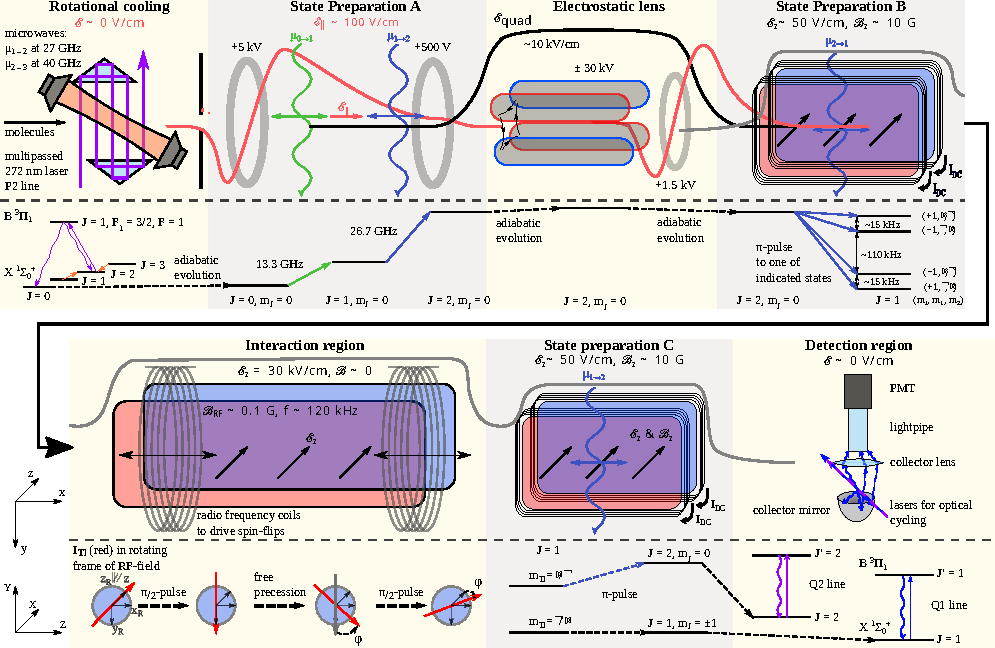
\includegraphics[width=\textwidth]{figs/fig6overview.pdf}
    \caption[Conceptual flow chart of the \CENTREX\ experiment]{Conceptual flow
    chart of the critical steps in \CENTREX, indicating the applied fields
    (below) and the quantum states (above). This is Fig.~6 from our overview
    paper \cite{grasdijk2021centrex}.}
    \label{conceptdiagram}
\end{sidewaysfigure}

\subsection{Overview of the \CENTREX\ scheme}
\label{introduction:overview}

Referring to Fig.~\ref{conceptdiagram}, we follow the molecules emerging from a
cryogenic buffer gas beam source, initially in a range of low-lying states with
an approximate temperature of 8~K \cite{grasdijk2021centrex}. In order to
facilitate transfer to the `science' state used for the spin precession
measurement, molecules first enter a rotational cooling region to accumulate
population in a single hyperfine and rotational level. Then, to limit the
spreading of the beam, the molecules get transferred to the lensing state in
state preparation region A (SPA) and focused by an quadrupole electrostatic
lens. Since the lens state is different from the interaction state, the
molecules are prepared into the correct hyperfine state in a two-state adiabatic
rapid passage machine, the state preparation region B. Afterwards, they fly
through the main interaction region with the standard Ramsey separated
oscillatory field configuration to excite the \gls{NMR} resonance. Finally, we
probe the resulting spin direction to determine the extent of the possible
dependence of the spin precession frequency on the interaction region electric
field direction. This is done in state preparation region C (SPC), where each
spin state is transferred to a different rotational state. Finally, the
rotational populations are read out with \gls{LIF} and optical cycling in the
fluorescence detection region. 

\paragraph{Rotational cooling (Fig.~\ref{scheme})}

Assuming a simple Boltzmann distribution at 8~K, almost 90\%\ of the molecules
have $J$ in the range from 0 to 3. To move these molecules to $J=0$, we first
set up microwave couplings $J=1\leftrightarrow2$ and $2\leftrightarrow3$. Then,
a \UV\ laser beam centered on the $P2$ $F1$ line (terminology defined on page
\pageref{P2F1}) lifts the population from $J=2$ into the excited state $J'=1$,
from where it decays down to either $J=0$ or $J=2$. Since the $J=2$ molecules
eventually get excited by the laser again, we expect the population to
accumulate in $J=0$.

The preceding description ignores the complications due to the hyperfine
structure. Since the excited state hyperfine levels are well separated (unlike
the unresolved \hfs\ of the electronic ground state), we can address the $F'=1$
level. Due to the selection rule $\Delta F=0,\pm1$, only three of the four $J=2$
sublevels (with $F=1,2,2$) can be excited into $J'=1$, from where they decay
into $J=0$ states with $F=1,0$. A further set of microwaves, between $J=0$ and
$J=1$, is used to remix the $F=1$ states, so as to concentrate the population
only in the $F=0$ state. (If we were to use the $P2$ $F2$ transition instead,
then it would be possible to excite all four $F$ sublevels of the $J=2$ state up
into a $F'=2$ level. However, the branching ratio---calculated using
eqn~\ref{branchingratios}---for decays to $F=0$ are vanishing from $F'=2$.)

As stated, the $P2$ $F1$ line (terminology defined on page \pageref{P2F1}) does
not excite the $F=3$ states, so these are trivially dark. But since there are
only 3 sublevels in $F'=1$, compared to the 20 sublevels in the $J=2$ manifold,
there is a total of 17 dark states, i.e.\ states which cannot be excited using
this laser transition \cite[sect~3.1.3]{barry2013thesis}. These dark states may
be destabilized \cite{berkeland2002destabilization} by frequency-switching
microwaves precisely tuned to the individual sublevels that cannot be resolved
by the laser light. This can also be done, as is the plan in this experiment, by
switching the polarizations of the laser and both microwave beams, and ensuring
that no pair of the three beams are either parallel or perpendicular to each
other.

\paragraph{State preparation A}

The population that has been collected in the $J=0$, $F=0$ sublevel has to be
moved to the state in the $J=2$ manifold chosen for the optimal operation of the
electrostatic lens (see next paragraph). We plan to accomplish the transfer as a
two-stage adiabatic rapid passage (\ARP): first $J=0\to1$, then $1\to2$. As the
particles travel through a spatially-varying electric field, the separation
between the hyperfine levels in the different $J$ states changes due to the \DC\
Zeeman effect. In the same region, we place two microwaves beams corresponding
to each pair of $J$ states, and offset them by approximately the \FWHM\ of each
beam. As the molecule traverses each beam, it is successively driven through
the respective microwave resonances, making the population jump first to $J=1$,
and then to $J=2$.

To keep the state transfer adiabatic, the electric field (and the resulting
level separation, and the detuning $\Delta\omega(t)$ between the microwaves and
the state spacing) has to change slowly compared with the Rabi frequency of the
microwaves $\Omega_{\mu\text{w}}$. For a Rabi frequency much greater than the
detuning, ref.~\cite{malinovsky2001general} gives the adiabaticity condition as
%
\[
\Omega^2_{\mu\text{w}}\gg\frac{d}{dt}\Delta\omega(t).
\]
%
The other requirement for \ARP\ is that the passage is \emph{rapid} compared to
the spontaneous lifetime of the states involved in the transition, which here is
effectively infinite. \cite{shore2009simple}

\begin{figure*}
    \centering
    \small
    \hfill
    \begin{minipage}[c]{0.4\textwidth}
        \begin{tikzpicture}

    % kets
    \node (J0)  at (0,0)   {$\ket{J=0}$};
    \node (J1)  at (2,.5)  {$\ket{J=1}$};
    \node (J2)  at (4,1)   {$\ket{J=2}$};
    \node (J3)  at (6,1.5) {$\ket{J=3}$};
    \node (Je1) at (3,4)   {$\ket{J'=1,F_1'=3/2,F'=1}$};

    % Boltzmann population at 8K
    \node[below=-5pt of J0] (p0) {\footnotesize31.4~\%};
    \node[below=-5pt of J1] (p1) {\footnotesize26.7~\%};
    \node[below=-5pt of J2] (p2) {\footnotesize19.4~\%};
    \node[below=-5pt of J3] (p3) {\footnotesize11.9~\%};

    % P2 F1 laser line
    \draw[-{Latex[length=4mm,width=4mm]},line width=3pt,gray] (4,1.25) -- node[above,black,sloped]{$P2$ $F1$} (3.25,3.75);

    % spontaneous decay branching ratios
    \tikzset{snake it/.style={-{Latex[length=2mm,width=2mm]}, decorate, decoration={snake,amplitude=2pt,pre length=2pt,post length=3pt}}}
    \draw[snake it] (2,3.75) -- node[left,xshift=-1pt] (num) {\footnotesize0.335} (0,.25);
    \node[above=0.2 of num] {\normalsize (a)};
    \draw[snake it,dashed] (2.5,3.75) -- node[left,yshift=8pt,xshift=2pt]{\footnotesize0.860} (2,.75);
    \draw[snake it] (2.75,3.75) -- node[left,xshift=3pt,yshift=-10pt]{\footnotesize0.665} (3.5,1.25);
    \draw[snake it,dashed] (4,3.75) -- node[right,xshift=3pt]{\footnotesize0.140} (6,1.75);

    % microwaves
    \tikzset{biarrow/.style={{Latex[length=1.5mm,width=1.5mm]}-{Latex[length=1.5mm,width=1.5mm]}}}
    \draw[biarrow,dashed] (p0) to[bend right] node[below,sloped]{\small13.4~GHz} (p1);
    \draw[biarrow] (p1) to[bend right] node[below,sloped]{\small26.6~GHz} (p2);
    \draw[biarrow] (p2) to[bend right] node[below,sloped]{\small40.1~GHz} (p3);

\end{tikzpicture}


    \end{minipage}
    \hfill
    \begin{minipage}[c]{0.4\textwidth}
        \input{figs/tikz/rothypF1.tex}
    \end{minipage}
    \hfill
    \mbox{}
    \caption[Proposed rotational cooling scheme.]{Proposed rotational cooling scheme. \part{a} The thick solid arrow marks the \UV\ laser driving the $P2$ $F1$ transition (terminology defined on page \pageref{P2F1}), while the bent arrows represent microwaves with the stated frequencies (the dashed 13.4~GHz microwaves might be omitted in the final version). The wavy arrows indicate spontaneous emission, with rotational branching ratios taken from ref.~\cite[Table~IV]{norrgard2017hyperfine}. The odd-parity $\Omega$-doublet excited state can only decay to the states with $J=0,2$ (solid wavy lines), and not the $J=1,3$ ones (dashed wavy lines), and the branching ratios are normalized to unity for each parity. The percentages under the ground-state kets are the expected thermal population at 8~K before beginning rotational cooling. \part{b} Hyperfine details of the rotational cooling scheme. Decays back to $J=2$ not shown here. The $P2$ $F1$ transition, shown here, does not couple to $F=3$. However, the $P2$ $F2$ line (not shown) that does couple to all $F$ has a vanishing branching ratio into $F=0$.}
    \label{scheme}
\end{figure*}

\paragraph{Electrostatic lens}

Molecules leave the beam source spread over a wide solid angle, so the beam
intensity decreases roughly as the distance squared from the source. To
counteract this effect, we intend to collimate the beam, or focus it on the
detection region, some seven meters away from the source.

It turns that that an appropriate field distribution can be used as an analogue
to the optical lens \cite{cho1991tight}, the condition being that inside the
lens, molecules experience a restoring force proportional to the displacement
$r$ of the molecule from the axis. For a quadrupole field, the magnitude of the
field is $|E|=Vr/R^2$, where $V$ is the potential difference between
oppositely-charged electrodes and $2R$ the distance between opposite electrodes.
\cite{bennewitz1955fokussierung} Furthermore, since the $J=2,m=0$ state of thallium
fluoride has a positive quadratic Stark shift even at high fields
($\propto30\kVcm$), this results in the desired quadratic potential energy, or a
linear restoring force.  Ref.~\cite{berg1965determination} makes the optical
analogy exact in terms of ray-transfer (or `ABCD') matrices, whereby the
condition for focusing results in the standard expression for a thin lens of
focal length $f$
%
\begin{align*}
    \begin{pmatrix}
        r\\
        \dot r/u
    \end{pmatrix}
    =
    \begin{pmatrix}
        1&0\\
        -1/f&1
    \end{pmatrix}
    \begin{pmatrix}
        r_0\\
        \dot r_0/u
    \end{pmatrix},
\end{align*}
%
where $u$ is the component of velocity along the beam direction (making $\dot
r_0/u$ proportional to the angle relative to the axis), and $r_0(t)$ the
pre-lens displacement of the molecule from the beam axis. The focal length for
molecules of mass $m$ is \cite[cf.\ eqn~12]{berg1965determination}
%
\[
    f=\frac{1}{p\sin pl},
    \quad
    p=-\frac{CV^2}{R^4mu^2},
\]
%
where $l$ is the length of the quadrupole lens, and $C$ is a constant encoding
the $J$, $m_J$ dependence of the quadratic Stark effect.

\paragraph{State preparation B}

A second state preparation region will take molecules out of the lens $J=2$
state and into the appropriate $J=1$ state required by the interaction region.
To achieve this, a resonant microwave field with  will be applied in the
presence of a magnetic field and a quantizing electric field. Since adiabatic
passage can drive undesired transitions to unwanted states nearby in energy,
here we use a microwave $\pi$-pulse to achieve optimized transfer efficiency.
The simulated transfer efficiency is approx.\ 96\%. In practice, the transfer
efficiency is likely to be reduced due to non-uniformities of the electric and
magnetic fields, since changes in the fields cause the transition frequencies to
shift away from the microwave frequency.  \cite[sect~2.5]{grasdijk2021centrex}

\paragraph{Interaction region}

\begin{figure}
    \centering
   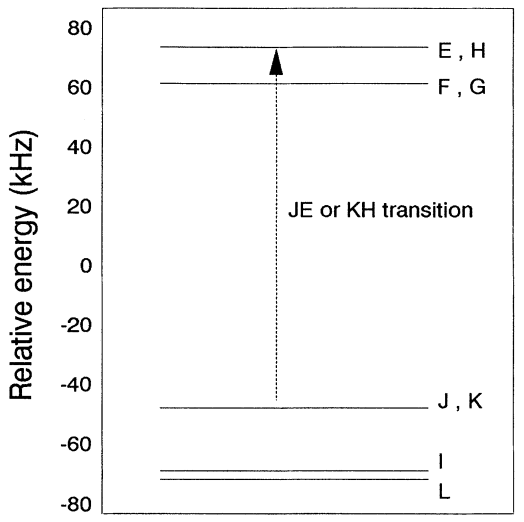
\includegraphics[width=.5\textwidth]{figs/todo/cho1991fig7.png}
    \caption[TlF hyperfine levels]{Hyperfine sublevels of $(J=1,M_J=\pm1)$ in an electric
    field of 29.5~kV/cm. Figure reproduced from Cho et al.\
    \cite[Fig.~7]{cho1991search}.}
  \label{cho1991fig7}
\end{figure}

\begin{sidewaystable}
    \small
    \makebox[\textwidth][c]{%
        \begin{tabu} to \textwidth {@{}r @{\hspace{3pt}} ccc cc ccc ccc ccc@{}}
        \toprule
              & \multicolumn{4}{c}{State 1} & \multicolumn{4}{c}{State 2} &
              \multicolumn{2}{c}{$|\bra{\cdot}\mathcal{H}_\text{Z}\ket{\cdot}|$
              [kHz/G]\hspace{1.5ex}\mbox{}} & $S_\text{\gls{SMT}}$ & $S^z_m$ & $f_0$ & $df_0/dE_z$ \\
                  \cmidrule(r{2.0ex}){2-5}\cmidrule(r{2.0ex}){6-9}\cmidrule(r{2.0ex}){10-11}
            What flips?\hspace{1ex} & $l_\text{R}$ & $m_J$ & $m_\text{Tl}$ & $m_\text{F}$ & $l_\text{R}$ & $m_J$ & $m_\text{Tl}$ & $m_\text{F}$ & $x,y$ & $z$ & --- & mHz/$\mu$G & kHz & mHz/(V/cm) \\
        \midrule
            \multirow{2}{*}{$m_\text{Tl}\;\Big\{$}             & e & $-$ & $-$ & $-$ & j & $-$ & $+$ & $-$ & \multirow{2}{*}{1.33} & \multirow{2}{*}{0.00} & \multirow{2}{*}{0.95} & \multirow{2}{*}{$5.0$} & \multirow{4}{*}{119.517} & \multirow{4}{*}{$31.50$} \\
                                                               & h & $+$ & $+$ & $+$ & k & $+$ & $-$ & $+$ &                       &                       &                       & \\
            \multirow{2}{*}{$m_J, m_\text{F}\;\Big\{$}         & e & $-$ & $-$ & $-$ & k & $+$ & $-$ & $+$ & \multirow{2}{*}{0.28} & \multirow{2}{*}{0.00} & \multirow{2}{*}{0.04} & \multirow{2}{*}{$8.1$} \\
                                                               & h & $+$ & $+$ & $+$ & j & $-$ & $+$ & $-$ &                       &                       &                       \\\dashedrule
                                                                                                                                                                                   
            \multirow{2}{*}{$m_J\;\Big\{$}                     & f & $+$ & $+$ & $-$ & j & $-$ & $+$ & $-$ & \multirow{2}{*}{0.00} & \multirow{2}{*}{0.00} & \multirow{2}{*}{0.00} & \multirow{2}{*}{$0.1$} & \multirow{4}{*}{108.924} & \multirow{4}{*}{$3.57$} \\
                                                               & g & $-$ & $-$ & $+$ & k & $+$ & $-$ & $+$ &                       &                       &                       \\
            \multirow{2}{*}{$m_\text{Tl}, m_\text{F}\;\Big\{$} & f & $+$ & $+$ & $-$ & k & $+$ & $-$ & $+$ & \multirow{2}{*}{0.00} & \multirow{2}{*}{0.09} & \multirow{2}{*}{0.99} & \multirow{2}{*}{$3.0$} \\
                                                               & g & $-$ & $-$ & $+$ & j & $-$ & $+$ & $-$ &                       &                       &                       \\\dashedrule
                                                                                                                                                                                   
            \multirow{2}{*}{$m_\text{F}\;\Big\{$}              & e & $-$ & $-$ & $-$ & g & $-$ & $-$ & $+$ & \multirow{2}{*}{1.88} & \multirow{2}{*}{0.00} & \multirow{2}{*}{0.04} & \multirow{2}{*}{$8.0$} & \multirow{4}{*}{10.593} & \multirow{4}{*}{$27.93$} \\
                                                               & h & $+$ & $+$ & $+$ & f & $+$ & $+$ & $-$ &                       &                       &                       \\
            \multirow{2}{*}{$m_J, m_\text{Tl}\;\Big\{$}        & e & $-$ & $-$ & $-$ & f & $+$ & $+$ & $-$ & \multirow{2}{*}{0.40} & \multirow{2}{*}{0.00} & \multirow{2}{*}{0.95} & \multirow{2}{*}{$5.0$} \\
                                                               & h & $+$ & $+$ & $+$ & g & $-$ & $-$ & $+$ &                       &                       &                       \\
        \bottomrule
    \end{tabu}}
    \caption[Nuclear transitions in TlF.]{All non-degenerate pairs of $|m_J|=1$
    states in the asymptotic $J=1$ manifold that do not involve the states
    $\ket{\text{i}}$ and $\ket{\text{l}}$. The quantum numbers given are that of
    the largest decoupled-basis component; states i and l have two such
    components with equal amplitude, making it hard to say what spin is flipped.
    The labels $l_\text{R}$ are as given in ref.~\cite{wilkening1984search} and
    Fig.~\ref{cho1991fig7}, above. The column labelled $S_\text{\gls{SMT}}$
    gives the sensitivity to the Schiff moment (eqn~\ref{ssmt}). The quantity
    $S^z_m$ gives the energy difference between the pair of resonances in a
    single row of the table, given per unit external residual $B_z$ Due to
    degeneracy of pairs $\mathrm{(e,h)}$, $\mathrm{(f,g)}$, and
    $\mathrm{(j,k)}$, there are only three distinct resonant frequencies $f_0$
    and slopes $df_0/dE_z$ at 30~kV/cm. All quantities (except quantum numbers)
    are given without their sign.}
    \label{statepairs}
\end{sidewaystable}


A high external electric field polarizes the molecules, thus enabling the linear
energy shift due to the Schiff moment. The measurement will be done using the
method of separated oscillatory fields as explained above.

We intend to use in this measurement a pair of $J=1$, $m_J=\pm1$ states, where
the molecular rotation leads to an internal magnetic field. By flipping the sign
of $m_J$, the internal magnetic field can be reversed. The first \RF\ coil in
the Ramsey sequence creates a superposition of thallium spin-up and spin-down
states, and the phase accumulated during the interaction time is translated by
the second pulse back into varying populations of the spin states. Data obtained
with the two different fluorine spin directions can be used for systematic
checks.

Refer to Table \ref{statepairs} and Fig.~\ref{cho1991fig7} for a list of all
available pairs of states we can make use of. For the \gls{EDM}\ measurement, of
course, only the transitions that flip the Tl nuclear spin are suitable. We
quantify the sensitivity $S_\text{\gls{SMT}}$ to the $T$-violating physics as
the extent to which the transition between states $i$ and $f$ flips the thallium
spin:
%
\begin{equation}
    \label{ssmt}
    S_\text{\gls{SMT}}\equiv
    |\ex{I_{1,z}}_i
    -
    \ex{I_{1,z}}_f|
\end{equation}
%
We can see that this quantity has a significant magnitude only for the three
pairs of transitions that are labelled as flipping $m_\text{Tl}$. Of these, the
first pair listed (ej/hk) is the one used in the papers by Ramsey et al.\
\cite{wilkening1984search} and Hinds et al.\ \cite{cho1991search} One pair of
transitions (ef/hg) has a much smaller resonant frequency than the other two,
but is otherwise comparable.

The quantity $S_m^z$ quantifies the sensitivity to the residual magnetic field
$B_z$ in the interaction region. For a pair of transitions $(i,j)$, where the
relevant quantum numbers ($m_J,m_1,m_2$) of the two states involved in $i$ are
reversed compared to the two states in $j$, we define
%
\[
    S_m^z\equiv
    \frac{\d(f_i-f_j)}{\d B_z},
\]
%
where $f_i,f_j$ are the resonant frequencies of the two transitions. In the
absence of $B_z$, the quantity should vanish, since the direction of the
internal molecular magnetic field $B_\text{mol}$ does not impact the eigenvalues
of the Hamiltonian. However, with a residual field $B_z$ present, the two
different signs of $B_\text{mol}$ form a sum and difference with $B_z$,
resulting in two different magnitudes of the overall magnetic field, and thus a
change in resonant frequencies $f_i$ and $f_j$.

In Table \ref{statepairs}, we see that the pair of transitions least sensitive
to $B_z$ is the one that only flips $m_J$ and leaves $m_1,m_2$ unchanged. The
next most `resilient' pair is fk/gj; that pair of transitions flips both the
thallium and the fluorine spins. The sensitivity to external fields is reduced
since the magnetic dipole moments of these nuclei are relatively well matched
\cite{stone2005table}:
%
\begin{align*}
    \mu(\ce{^{205}_{81}Tl})&=+1.63821461(12)\mu_\text{N}\\
    \mu(\ce{^{19}_{9}F})&=+2.628868(8)\mu_\text{N}.
\end{align*}

Of the three pairs of transitions that do not flip $m_\text{Tl}$, the pair fj/gk
is exactly forbidden. The other two (ek/hj and eg/hf) are about as sensitive to
field imperfections as the two pairs of $m_\text{Tl}$-flipping transitions ej/kh
and ef/hg, but $\approx23$ times less sensitive to the $T$-violating physics.
These states can thus be used for magnetometer/electrometer transitions in
calibrating the experimental systematics.

There are a further 13 possible transitions, not listed in Table
\ref{statepairs}, involving the `superposition' states $\ket{\text{i}}$ and
$\ket{\text{l}}$, given in \cite[Table~I]{cho1991search} with the following
$\ket{m_J,m_1,m_2}$ eigenvectors:
%
\[
    \ket{\text{i}},\ket{\text{l}}
    =
    \frac{1}{\sqrt2}
    \big(
    \,
        \ket{+,-,-}\pm\ket{-,+,+}\
    \big).
\]
%
These states can be ignored, since only one ket of the pair flips the thallium
spin when transitioning to a non-superposition state, and as such can be only
half as sensitive to $T$-violating physics. On the other hand, the transition
between $\ket{\text{i}}$ and $\ket{\text{l}}$ does not flip $m_\text{Tl}$ at
all.

\paragraph{State preparation C}

Before the molecular states can be probed in the detection region, we have to
map the two spin states---which cannot be distinguished optically---from the
interaction region to two different rotational states using microwaves. In
contrast, different rotational states are spectrally resolvable by a probing
laser. This will allow optical detection of each original spin-state population.
\cite[sect~2.7]{grasdijk2021centrex} An optimized scheme for this state transfer
mechanism is currently being investigated, but the principle will likely be
analogous to SPC.

\paragraph{Detection}

Unlike some of the experiments discussed above, \CENTREX\ will employ
laser-induced fluorescence (\LIF) to detect the number of molecules in the final
rotational states. Compared to hot-wire or absorption techniques, \LIF\ has the
advantage of observing a signal against a dark background (modulo light
scattered from the optics and vacuum chamber windows).
\cite{tango1968spectroscopy} Furthermore, since the emitted light can be
collected at different angles, we can obtain spatial information about the
detection process. \cite{zare2012my}

To improve detection efficiency, we will use optical cycling to maximize the
number of emitted photons from each molecule. This cycling, which has been
demonstrated experimentally in TlF
\cite{clayburn2019optical,clayburn2021improved,clayburn2022improved}, will allow
for near unit-efficiency detection of each molecule.

The rotational sublevels of the TlF ground state are far enough apart to require
two detection lasers. Rapid switching between the lasers will allow for
quasi-simultaneous readout of both the spin-up and spin-down populations in a
single molecular-beam pulse, minimizing the effect of molecule number
fluctuations within and between pulses \cite{kirilov2013shot}. The switching, to
be accomplished with acousto-optic modulators, will allow enough dead time
between switches for the excited state to decay, but also will be rapid enough
such that each molecule sees both laser frequencies multiple times while
traveling through the optical interaction region. A similar scheme is
implemented by the ACME experiment \cite{acme2018improved}.

The resulting fluorescence will be collected by a combination of high numerical
aperture lenses and mirrors to cover a total solid angle of approx.\
$0.3\times4\pi$~sr. With PMT quantum efficiency of 25\%, each emitted photon
will then be detected with 7.5\% efficiency. Hence, scattering 30 photons per
molecule will be sufficient that each molecule is detected with 90\%
probability. Based on known branching ratios for decay out of each cycling
transition in TlF \cite{norrgard2017hyperfine}, this should be feasible.

The fluorescence signals $\mathrm{S}_\uparrow$ and $\mathrm{S}_\downarrow$,
corresponding to populations in the Tl spin-up and spin-down states after the
\gls{SOF} sequence, are then used to compute the asymmetry $\mathcal{A}$,
defined as:
%
\begin{equation}
    \mathcal{A}\equiv\frac{\mathrm{S}_\uparrow-\mathrm{S}_\downarrow}{\mathrm{S}_\uparrow+\mathrm{S}_\downarrow}.
\end{equation}

\subsection{Conclusion}

\keypoint{What have we learned here?}

In this chapter, we have learned about some of the unsolved mysteries of nature
that motivate an inquiry into processes that bring about a violation of the
fundamental symmetries. We have defined a quantity called the Schiff moment,
which represents a measurable consequence of new $T$-violating phenomena. We
have seen some of the advantages of using molecules to probe into the new
physics. This is the approach taken in a line of experiments spanning the
decades before the present work. We have also reviewed how our current
experiment continues the exploration in the direction of stricter bounds on the
scale of $T$-violating phenomena.

\keypoint{Why is it important for CeNTREX?}

These preliminary observations are important to understand the \CENTREX\
experiment. Despite its small scale compared to typical high energy physics
experiments, our experiment consists of a number of modules relying on modern
atomic and molecular physics techniques.

\keypoint{Will we revisit it in later sections?}

In this thesis, we will be exploring the experimental apparatus in greater
detail in chapter~\ref{ch_app}. The sections that the author of the present
manuscript has been more significantly involved with will be explored in greater
depth. These include especially the beam source (chapter~\ref{beam_source_ch})
and the magnetic shield (chapter~\ref{mfc_chapter}), as well as selected topics
related to the rotational cooling (chapter~\ref{RC_chapter}), a scaled-down
model of the interaction region (chapter~\ref{test_int_ch}), the high-voltage
system for the interaction region and the lens (chapter~\ref{HV_chap}) as well
as the lens itself (chapter~\ref{lens_ch}).

\keypoint{What are the biggest remaining challenges to getting a measurement?}

This chapter introduced the basic principles behind the measurement proposed by
the \CENTREX\ collaboration. On a level of a high-level overview as seen here,
there are no major theoretical obstacles to conducting the measurement. However,
in later sections we will meet some of the practical problems that need to be
addressed before a measurement can be obtained.
